%% ==========================================================
%%  Water as Strategy
%%  A Double Materiality Framework for Aqualia, 2027–2030
%%
%%  Los Gatos de Datos — IE Sustainability Datathon, March 2026
%%  Compile with:  latexmk -xelatex thesis.tex
%% ==========================================================

\documentclass[11pt, a4paper, twoside, openright]{scrreprt}

%% -------- Fonts & typography -------------------------------
\usepackage[utf8]{inputenc}
\usepackage[T1]{fontenc}
\usepackage{lmodern}        % modern serif
\usepackage{helvet}         % sans (Helvetica-clone)
\usepackage{courier}        % mono
\usepackage{textcomp}
\usepackage{microtype}
\usepackage{setspace}
\usepackage{amsmath}
\usepackage{amssymb}
\onehalfspacing

%% -------- Geometry -----------------------------------------
\usepackage[a4paper,
  inner=3.0cm, outer=2.5cm,
  top=2.8cm, bottom=2.8cm,
  headheight=14pt, headsep=18pt,
  footskip=22pt]{geometry}

%% -------- Colours ------------------------------------------
\usepackage[table, dvipsnames]{xcolor}
\definecolor{navy}{HTML}{002F5F}
\definecolor{deep}{HTML}{0B4F74}
\definecolor{aqua}{HTML}{5DB9D9}
\definecolor{sand}{HTML}{D6CDB7}
\definecolor{slate}{HTML}{4A5663}
\definecolor{ink}{HTML}{2C333B}
\definecolor{grid}{HTML}{E6E8EB}
\definecolor{t1col}{HTML}{1F77B4}
\definecolor{t2col}{HTML}{FF7F0E}
\definecolor{t3col}{HTML}{2CA02C}
\definecolor{badred}{HTML}{C83C35}
\definecolor{amber}{HTML}{F2B039}

%% -------- Headings / chapter style -------------------------
\usepackage[explicit]{titlesec}

\titleformat{\chapter}[display]
  {\normalfont\sffamily}
  {\color{aqua}\fontsize{9pt}{9pt}\selectfont\bfseries
    CHAPTER \thechapter\hspace{0.8em}\textcolor{grid!70!white}{\rule[0.35ex]{6cm}{0.6pt}}}
  {1em}
  {\color{navy}\fontsize{28pt}{32pt}\selectfont\bfseries #1}
\titlespacing*{\chapter}{0pt}{0pt}{1.6cm}

\titleformat{\section}
  {\normalfont\sffamily\large\bfseries\color{navy}}
  {\thesection}{0.6em}{#1}
\titlespacing*{\section}{0pt}{1.2em}{0.5em}

\titleformat{\subsection}
  {\normalfont\sffamily\normalsize\bfseries\color{ink}}
  {\thesubsection}{0.6em}{#1}
\titlespacing*{\subsection}{0pt}{0.9em}{0.3em}

\titleformat{\subsubsection}
  {\normalfont\sffamily\small\bfseries\color{slate}}
  {}{0em}{#1}

%% -------- Header / footer ----------------------------------
\usepackage{fancyhdr}
\pagestyle{fancy}
\fancyhf{}
\renewcommand{\headrulewidth}{0pt}
\renewcommand{\footrulewidth}{0pt}

\fancyfoot[LE,RO]{\small\color{slate}\thepage}
\fancyfoot[RE,LO]{\small\color{slate}\textsf{Water as Strategy\ \ \textbullet\ \ Los Gatos de Datos}}

\fancyhead[LE,RO]{\small\sffamily\color{slate}\leftmark}
\fancyhead[RE,LO]{}

%% -------- Tables & boxes -----------------------------------
\usepackage{booktabs}
\usepackage{tabularx}
\usepackage{array}
\usepackage{longtable}
\usepackage{multirow}
\usepackage{tcolorbox}
\tcbuselibrary{skins,breakable}

\newtcolorbox{callout}[1][]{
  enhanced, breakable,
  colback=grid!40!white, colframe=aqua, boxrule=0pt,
  leftrule=3pt, left=10pt, right=10pt, top=8pt, bottom=8pt,
  fontupper=\small, #1
}

\newtcolorbox{insight}[1][]{
  enhanced, breakable,
  colback=navy, coltext=white, colframe=navy, boxrule=0pt,
  left=12pt, right=12pt, top=10pt, bottom=10pt,
  fontupper=\small, arc=4pt,
  #1
}

%% -------- Hyperlinks ---------------------------------------
\usepackage[colorlinks=true,
  linkcolor=navy, citecolor=deep, urlcolor=deep,
  pdftitle={Water as Strategy — Aqualia Double Materiality 2027–2030},
  pdfauthor={Los Gatos de Datos},
  pdfsubject={CSRD-aligned Double Materiality Assessment for Aqualia},
  pdfkeywords={CSRD, ESRS, double materiality, water utility, Aqualia, Monte Carlo, Mitchell-Agle-Wood}
]{hyperref}

%% -------- Lists & misc -------------------------------------
\usepackage{enumitem}
\setlist{itemsep=2pt, topsep=4pt, parsep=0pt}

\usepackage{graphicx}
\graphicspath{{./figures/}{../04_matrix/}{../10_dashboard/}}

\usepackage[font=small, labelfont={bf, color=navy}, textfont=it, labelsep=period, justification=justified]{caption}

\usepackage{epigraph}
\setlength{\epigraphwidth}{0.85\textwidth}

\usepackage{csquotes}

%% -------- Bibliography ------------------------------------
%% Using natbib + bibtex for maximum portability (no biber dependency).
\usepackage[numbers, sort&compress]{natbib}

%% -------- Custom commands ----------------------------------
\newcommand{\euro}{\texteuro}
\newcommand{\signalword}[1]{\textbf{\textcolor{navy}{#1}}}
\newcommand{\note}[1]{{\footnotesize\textit{\textcolor{slate}{#1}}}}

%% ==========================================================
\begin{document}

%% -------- Title page ---------------------------------------
\begin{titlepage}
\thispagestyle{empty}

\vspace*{1.6cm}

{\sffamily\color{aqua}\bfseries\large IE SUSTAINABILITY DATATHON \textbullet\ MARCH 2026}
\par\vspace{0.3cm}
\textcolor{aqua}{\rule{\textwidth}{1.2pt}}
\par\vspace{2.6cm}

{\fontsize{56pt}{60pt}\selectfont\sffamily\bfseries\color{navy} Water as}\par
\vspace{0.2cm}
{\fontsize{56pt}{60pt}\selectfont\sffamily\bfseries\color{aqua} Strategy.}\par

\vspace{1.2cm}
{\Large\sffamily\color{deep} A Double Materiality Framework for\\ Aqualia, 2027--2030}\par

\vspace{2.0cm}
{\large\color{ink} Three material topics. A \euro{}500~million EU-Taxonomy-aligned green bond programme. A 2027--2030 strategic roadmap with named owners and measurable~KPIs.}\par

\vspace{0.6cm}
{\normalsize\color{slate} Simulated external ESG advisory engagement for Aqualia, the integrated water-cycle operator of the FCC Group. Serving approximately 32~million users across eight countries.}\par

\vfill

\textcolor{navy}{\rule{\textwidth}{0.8pt}}
\par\vspace{0.5cm}

\noindent
\newcommand{\tplabel}[1]{\parbox[t]{3.2cm}{\small\sffamily\bfseries\color{aqua}#1}}
\newcommand{\tpvalue}[1]{\parbox[t]{12cm}{\color{navy}#1}}

\tplabel{TRACK}\tpvalue{Double Materiality \& ESG Strategy $\cdot$ Aqualia}\par\smallskip
\tplabel{TEAM}\tpvalue{Los Gatos de Datos $\cdot$ IE Master in Business Analytics \& Data Science}\par\smallskip
\tplabel{LIVE DECK}\tpvalue{\ttfamily ma731.github.io/Aqualia-Datathon}\par\smallskip
\tplabel{DATE}\tpvalue{March 2026}\par

\end{titlepage}

%% -------- Front matter -------------------------------------
\pagenumbering{roman}

\chapter*{Abstract}
\addcontentsline{toc}{chapter}{Abstract}

\noindent
Aqualia, the integrated water-cycle operator of the FCC Group, serves approximately 32~million users across eight countries. Its 2025 double materiality review identified sixteen material topics and eighty-three specific impacts, risks, and opportunities (IROs). This thesis, prepared under a simulated external ESG advisory engagement for the IE Sustainability Datathon, reduces those sixteen topics to three, scores each under a CSRD/ESRS-aligned methodology, and translates the analysis into a 2027--2030 strategic roadmap with a corresponding funding instrument.

\medskip
The short-list---\emph{Water Resilience and Equitable Access}, \emph{Digital and Cyber Infrastructure}, and \emph{Green Finance and Integrity}---absorbs 73~percent of Aqualia's 83 IROs and holds its matrix position across four alternative stakeholder-weighting schemes (zero ranking flips). Three findings emerge. First, digitalisation is under-weighted: Aqualia's 2025 framework assigns only two of 83 IROs to it, the lowest count across a five-utility peer benchmark. Second, an equity signal is masked: customer satisfaction ranges 86--98~percent across six European and institutional markets, against 33~percent in Colombia---a 55-point spread compressed into a single group-level metric under ESRS~S4. Restoring ESRS~S3 (affected communities) as a standalone disclosure is our first recommendation. Third, Aqualia's existing lead on EU Taxonomy alignment is not quantified in capital-markets terms.

\medskip
Methodologically, we preserve Aqualia's published scoring structure (Severity $\times$ Probability) so results are directly comparable to their internal review, and extend it along four dimensions: \emph{(i)}~threshold calibration cited to ESRS, EFRAG, SASB, WRI Aqueduct, and MSCI; \emph{(ii)}~stakeholder salience weighting via the Mitchell--Agle--Wood (1997) model; \emph{(iii)}~a 10{,}000-draw Monte Carlo producing 90\% $\chi^2$ confidence ellipses; and \emph{(iv)}~a bilingual TF--IDF ESRS disclosure-gap heatmap across 873 paragraph chunks of Aqualia's 2022--2025 reports.

\medskip
The recurring annual financial materiality the current framework leaves un-priced, aggregated across the three topics, is \euro{}18~million per year. The implied 2027--2030 CAPEX is \euro{}440~million base case. We recommend funding via a \euro{}500~million EU-Taxonomy-aligned green / sustainability-linked bond programme issued in four tranches aligned to CAPEX drawdown. At the 2024 Climate Bonds Initiative-reported 25~basis-point green spread over vanilla investment-grade Euro water-utility issuance, the programme captures approximately \euro{}31~million of present-value interest savings over its ten-year life.

\vfill

\noindent\textbf{Keywords.} CSRD; ESRS; double materiality; water utility; Aqualia; Monte Carlo; Mitchell--Agle--Wood stakeholder salience; TF--IDF; EU Taxonomy; green bonds; climate adaptation.

\cleardoublepage
\tableofcontents
\cleardoublepage

%% -------- Main body ----------------------------------------
\pagenumbering{arabic}
\setcounter{page}{1}

\chapter{Introduction}
\label{chap:intro}

\epigraph{\itshape Water is no longer infrastructure. It is strategy.}{\textemdash{} Working thesis of this report}

\section{Context}

The Corporate Sustainability Reporting Directive~\cite{csrd2022} constitutes the most consequential reform of European corporate disclosure in two decades. Approximately 50{,}000 undertakings now fall inside its perimeter, with disclosure obligations operationalised across twelve topical standards in the European Sustainability Reporting Standards~\cite{esrs2023}. Two perspectives are mandatory: \emph{impact materiality}, covering how an undertaking affects society and the environment; and \emph{financial materiality}, covering how sustainability factors affect the undertaking's revenues, costs, assets, liabilities, and enterprise value. Together these perspectives form the regime known as \signalword{double materiality}.

For a water utility, double materiality sits unusually close to the operating core. Water is both the product and the environmental resource on which the product depends. A concession's reliability is a social obligation; its capital efficiency is a financial one; its exposure to climate-driven scarcity is increasingly both. The double materiality framework is accordingly a live strategic instrument for a water utility in a way that it may not yet be for issuers in other sectors.

\section{Aqualia}

Aqualia is the integrated water-cycle operator of the FCC Group. Its activity covers sourcing of raw water, potable treatment, distribution, sewerage, wastewater treatment, and the growing share of recycled water across Spain, Portugal, Italy, France, the Czech Republic, Colombia, and several project-operation markets. Aqualia's public disclosures~\cite{aqualiaSR2024} cite 130~years of operating record, service to more than 32~million users, and \euro{}40~million per year of sustained infrastructure investment.

Aqualia's 2025 Sustainability Report \cite{aqualiaSR2024} discloses total revenue-volume of business of \euro{}1{,}674.7~million for financial year 2024, of which 98.8~percent is EU-Taxonomy eligible and 45.74~percent Taxonomy aligned (p.~103). This places Aqualia in the upper quartile of Spanish water utilities on Taxonomy alignment and creates a concrete, as-yet-unmonetised opportunity in the capital markets.

\section{Commission}

We operate as an external ESG advisory team. Our deliverable simulates the type of engagement Aqualia's executive committee or sustainability board would commission from a consultancy: consolidated topic selection, explicit scoring methodology, an auditable matrix, and an actionable 2027--2030 roadmap.

The starting point is Aqualia's 2025 comprehensive Double Materiality Review \cite{aqualiaDMReview2025}, which identifies sixteen material topics grouped into environmental (6), social (5), and governance (5) domains, and catalogues eighty-three IROs across the stakeholder ecosystem. The 2025 review is, in our assessment, one of the most thorough double materiality exercises in the Spanish water sector. It is also, in our view, too broad to drive a four-year strategic plan: sixteen equal priorities is operationally indistinguishable from none.

Our task, therefore, is not to start over. It is to sharpen. We reduce sixteen topics to three, score each with a methodology designed to withstand executive-committee review, and translate the analysis into a funded, scheduled roadmap.

\section{Thesis statement}

Three material topics---\signalword{Water Resilience and Equitable Access}, \signalword{Digital and Cyber Infrastructure}, and \signalword{Green Finance and Integrity}---absorb 73~percent of Aqualia's 83~IROs and hold their matrix position across four alternative stakeholder-weighting schemes. Recurring annual financial materiality the current framework leaves un-priced, aggregated across these three topics, is \euro{}18~million per year. A \euro{}500~million EU-Taxonomy-aligned green bond programme, issued in four tranches, funds the implied \euro{}440~million 2027--2030 CAPEX and captures approximately \euro{}31~million of present-value interest savings at the prevailing 25 basis-point green-bond spread.

\section{Structure of this thesis}

Chapter~\ref{chap:context} situates the work within CSRD, ESRS, and the broader regulatory landscape and documents Aqualia's operating context. Chapter~\ref{chap:methodology} specifies the four-phase methodology blueprint and the four extensions we apply to Aqualia's own scoring structure. Chapter~\ref{chap:topics} explains the topic-selection analytical funnel and justifies the three-topic short-list. Chapters~\ref{chap:impact} and~\ref{chap:financial} assess impact and financial materiality respectively. Chapter~\ref{chap:matrix} presents the matrix, its sensitivity drivers, and its stability across alternate stakeholder schemes. Chapter~\ref{chap:roadmap} develops the 2027--2030 strategic roadmap and the capital-markets instrument that funds it. Chapter~\ref{chap:limits} catalogues limitations and a reverse stress test. Chapter~\ref{chap:conclusion} concludes.

%% ==========================================================
\chapter{Regulatory and Commercial Context}
\label{chap:context}

\section{The CSRD / ESRS mandate}

The Corporate Sustainability Reporting Directive elevates sustainability reporting from a peripheral compliance activity to a bidirectional disclosure regime. Under CSRD, large undertakings must perform a double materiality assessment reporting both how their activities impact society and the environment (impact materiality, or ``inside-out'') and how ESG factors influence their financial performance and enterprise value (financial materiality, or ``outside-in''). The European Sustainability Reporting Standards~\cite{esrs2023} operationalise the Directive across twelve topical standards (E1--E5, S1--S4, G1) and a cross-cutting set of approximately 1{,}144 datapoints documented in EFRAG Implementation Guidance~\cite{efrag2024}.

Parallel regulation reinforces the CSRD core. The Corporate Sustainability Due Diligence Directive~\cite{csddd2024} imposes civil liability on large undertakings for supply-chain human-rights and environmental failings. The recast Urban Wastewater Treatment Directive \cite{uwwtd2024} introduces new obligations for emerging-pollutant removal and energy neutrality at wastewater treatment plants. In Spain, Real Decreto 1985/2024 \cite{rd1985} establishes a framework for the reuse of treated wastewater that materially affects Aqualia's reuse strategy.

The broader strategic overlay is the EU Water Resilience Strategy~\cite{waterResilience2025}, which names \emph{digitalisation of water infrastructure} as Action Area~3 of 5 and explicitly links water resilience to Europe's industrial competitiveness agenda.

\section{Aqualia's operating context}

Aqualia runs the full urban water cycle: sourcing raw water, treating it to drinking-water standard, distributing it to households and commercial customers, collecting sewage, operating wastewater treatment plants, and recycling treated water back into irrigation, industrial, and, increasingly, potable reuse applications. Operations span Spain, Portugal, Italy, France, the Czech Republic, Colombia, and a series of project-operation markets in the Middle East and elsewhere. Figure~\ref{fig:valuechain} shows the full value chain as Aqualia disclosed it in their 2025 corporate-context document.

\begin{figure}[htbp]
\centering
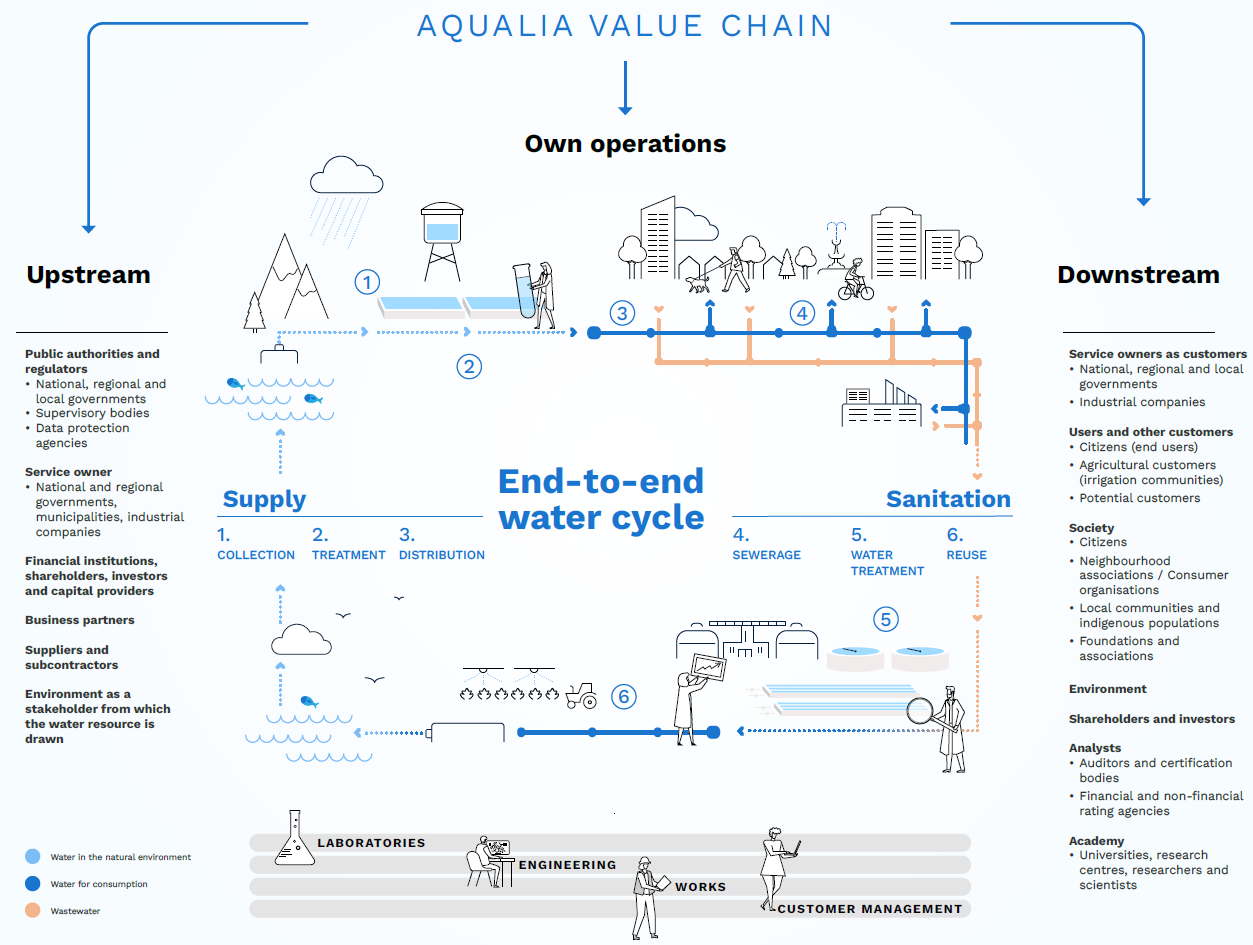
\includegraphics[width=\textwidth]{aqualia_value_chain.png}
\caption[Aqualia value chain]{Aqualia value chain, end-to-end urban water cycle. Upstream (suppliers, public authorities), own operations (seven steps from supply to sanitation), downstream (customers, affected communities). Source: Aqualia, \emph{Corporate Context and Sustainability Framework}~\cite{aqualiaSR2024}.}
\label{fig:valuechain}
\end{figure}

Three structural features bear on materiality. First, a \signalword{long-dated concession model}: contracts commonly span 15--30~years, which amplifies the financial consequences of both stranded assets and reputational damage. Second, \signalword{geographic exposure to climate-physical risk}: roughly 45~percent of revenue sits in basins classified as High or Extremely High water-stress under WRI Aqueduct~4.0, rising to approximately 79~percent under a BAU-2030 scenario~\cite{aqueduct2023}. Third, \signalword{regulatory density}: CSRD, UWWTD, RD~1985/2024, CSDDD, NIS2, and the EU Taxonomy all carry binding operational implications. A well-specified double materiality framework carries, in these conditions, the most decision-value.

\section{Framework boundary}

We take ESRS~1 and ESRS~2 cross-cutting standards plus the ten topical standards (E1--E5, S1--S4, G1) as the universe of candidate topics. Where Aqualia's 2025 review introduces sector-specific ``AQ''-prefixed topics (Technological Innovation, Digitalisation, Green Finance, Cybersecurity), we preserve those extensions. We overlay three complementary frameworks: the Taskforce on Nature-related Financial Disclosures~\cite{tnfd2023}, to which Aqualia has publicly committed; the SASB Water Utilities and Services standard~\cite{sasb2024}, as a sector-specific metric source; and the EU Taxonomy Regulation \cite{taxonomy2020} for CAPEX/OPEX alignment. We explicitly exclude sector-adjacent issues without a CSRD-compliant disclosure home, such as lobbying expenditure outside G1-5 coverage.

%% ==========================================================
\chapter{Methodology}
\label{chap:methodology}

\epigraph{\itshape We did not assert. We modelled.}{}

\section{Four-phase blueprint}

The work follows the four-phase blueprint adopted at the datathon's opening workshop: Phase~1 Context Analysis (peer benchmark, regulatory scan, internal baseline); Phase~2 Impact Materiality; Phase~3 Financial Materiality; Phase~4 Strategic Synthesis. Each phase produces a documented artefact that is subject to one independent team review before the next begins.

\section{Scoring formulas}
\label{sec:scoring}

We preserve the structural formulas Aqualia publishes in its own internal methodology~\cite{aqualiaMethodology2025}, with the explicit design goal that our output remains directly comparable to Aqualia's own 2025 review.

\subsubsection{Impact materiality}

\[
\text{Severity} = \tfrac{1}{3}\left(\text{Scale} + \text{Scope} + \text{Remediability}\right), \qquad \text{each rated } 1\text{--}5.
\]

Current impacts score Severity $\times\,5$ (probability pinned at maximum). Potential impacts score Severity $\times$ Probability. Raw scores fall in $[1, 25]$ and are linearly rescaled to $[1, 5]$.

\subsubsection{Financial materiality}

\[
\text{Severity}_{\text{fin}} = \text{Magnitude} \times \text{Probability} \times \text{Horizon Discount}.
\]

Magnitude is rated 1--5 against EFRAG thresholds and Aqualia's revenue proxy (see Section~\ref{sec:thresholds}). Probability uses the same 1--5 scale as impact. The horizon discount is 1.00 for the short term ($\leq 3$~years), 0.80 for medium (3--10~years), and 0.60 for long ($>10$~years), mirroring EFRAG Implementation Guidance~IG-1~\S69 on present-value framing.

\subsubsection{Topic aggregation}

Topic-level Impact or Financial score equals the mean of the top-$k$ IRO or R\&O scores, where $k = \max(3,\ \operatorname{round}(N \times 0.6))$. Top-$k$ aggregation mirrors standard practice of pricing materiality off the most material subset rather than an undifferentiated mean.

\subsubsection{Terminology mapping to the Datathon brief}

The Datathon brief (\S 3) lists four impact-materiality factors: \emph{scale, scope, likelihood, irreversibility}. Our formulas preserve Aqualia's published nomenclature. The mapping is one-to-one:

\begin{center}
\small
\begin{tabular}{@{}l l p{6.5cm}@{}}
\toprule
\textbf{Brief term} & \textbf{Our term} & \textbf{Relationship} \\
\midrule
Scale & Scale & identical \\
Scope & Scope & identical \\
Likelihood & Probability & synonymous ($P[\text{occur}]$ on the 1--5 scale) \\
Irreversibility & Remediability & inverse \\
\bottomrule
\end{tabular}
\end{center}

The factor \emph{set} is identical to the brief; the aggregation \emph{pattern} follows Aqualia's published practice rather than a single 4-factor mean. The Monte Carlo pipeline propagates uncertainty in all four factors simultaneously.

\section{Threshold calibration}
\label{sec:thresholds}

Threshold bands for every sub-criterion are documented in the scoring rubric and reproduced in Appendix~A. Anchors include ESRS~1~\S 43--51, EFRAG~IG-1~\cite{efrag2024}, SASB Water Utilities metrics \cite{sasb2024} (non-revenue water, pipe replacement, effluent non-compliance), WRI Aqueduct population-exposure bands~\cite{aqueduct2023}, and MSCI's 2024 Water Utilities sub-weights~\cite{msci2024}.

The Financial Magnitude scale is anchored to Aqualia's 2024 revenue. Our base case uses \euro{}1.4~billion (Assumption~A01) as a conservative proxy derived from FCC Group segment disclosure. Aqualia's 2024 Sustainability Report (p.~103) discloses a total revenue-volume of business of \euro{}1{,}674.7~million~\cite{aqualiaSR2024}, of which 98.8~percent is EU-Taxonomy eligible and 45.74~percent Taxonomy aligned. The conservative \euro{}1.4~billion anchor sits inside our published $\pm 20\%$ sensitivity band, and Section~7 of the financial workings confirms that the rank ordering of topics and the sign of the \euro{}18~million per year headline are stable under both anchors.

Band~3 (Moderate) corresponds to 0.5--2~percent of revenue (\euro{}7--28~M at the conservative anchor; \euro{}8--33~M at the disclosed anchor): a material budget line but recoverable from normal operations. Band~5 (Severe) exceeds 5~percent (\euro{}70~M conservative; \euro{}84~M disclosed): enterprise-level impact.

\section{Stakeholder salience}
\label{sec:salience}

Aqualia's 2025 review was scored internally by its Sustainability Department without external stakeholder consultation, as Aqualia's methodology acknowledges~\cite{aqualiaMethodology2025}. We restore a salience input by applying the Mitchell--Agle--Wood (1997) model~\cite{mitchell1997}, the canonical framework in stakeholder theory, to Aqualia's own ten-group stakeholder map. Each stakeholder is scored~$0/1$ on Power, Legitimacy, and Urgency; the salience score~$\in \{0,1,2,3\}$ becomes a normalised weight in $[0, 1]$ summing to 1.000.

Four stakeholder groups reach Definitive status (all three attributes present) in Aqualia's ecosystem: Public authorities and regulators; Customers and end-users; Shareholders; and Employees. Each carries weight 0.120. Six additional groups reach Expectant status (two attributes), each carrying weight 0.080: Investors, Suppliers, Business partners, Society/NGOs/media, Local communities, and Environment. Academia reaches Discretionary status (Legitimacy only) with weight 0.040. The full scoring table is reproduced in Appendix~F.

The underlying stakeholder map is Aqualia's own, reproduced in Figure~\ref{fig:stakeholders}. Columns describe each group's expectations, commitments, communication channels, and forums. We derive the Power / Legitimacy / Urgency attribute scores from the intensity and formality evident in each column (regulatory obligations map to Power; formal commitments map to Legitimacy; channel cadence and responsiveness expectations map to Urgency).

\begin{figure}[htbp]
\centering
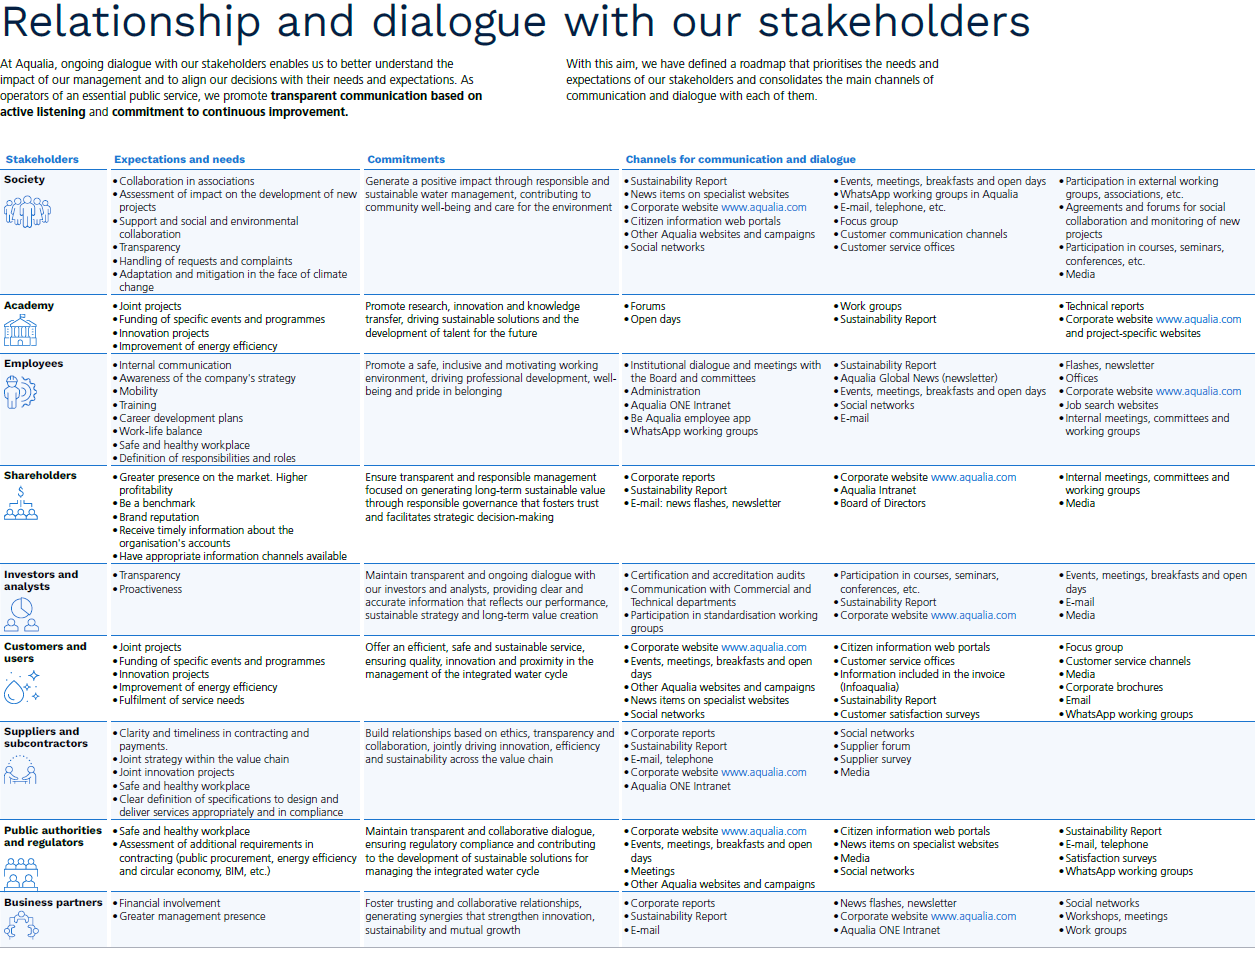
\includegraphics[width=\textwidth]{aqualia_stakeholder_map.png}
\caption[Aqualia stakeholder map]{Aqualia's own stakeholder ecosystem map, drawn from the 2025 Sustainability Report. Rows are stakeholder groups; columns capture expectations, commitments, channels, and forums. We apply the Mitchell--Agle--Wood salience model \cite{mitchell1997} directly to this taxonomy. Source: Aqualia~\cite{aqualiaSR2024}.}
\label{fig:stakeholders}
\end{figure}

\section{Monte Carlo design}
\label{sec:mc}

Every uncertain input feeds a triangular distribution centred on the base value with perturbation $\pm 0.7$ on the 1--5 score scale, clipped to $[1, 5]$. Stakeholder weights sample from a Dirichlet distribution centred on the salience vector with concentration parameter $\kappa = 100$. Financial magnitude uses a triangular distribution with topic-specific (low, base, high) parameters from the assumption log (Appendix~B).

Ten thousand draws are generated per topic. For each topic, the (Financial, Impact) scatter produces a 2D distribution from which a 90~percent $\chi^2$-containment confidence ellipse is drawn via eigendecomposition of the covariance matrix (containment constant $\chi^2_{2, 0.90} \approx 4.605$; the $1\sigma$ semi-axis scales by $\sqrt{4.605} \approx 2.146$ in each direction). The rendered matrix is reproduced in Figure~\ref{fig:matrix}.

\section{Robustness and sensitivity}

The Monte Carlo is repeated under four alternate stakeholder-weighting schemes: Equal (all eleven groups at $1/11$); Regulator-heavy (Public Authorities at 0.30); Community-first (Society $+$ Local Communities combined at 0.30); and Investor-first (Shareholders $+$ Investors combined at 0.40). No ranking flip occurs across schemes: T1 and T2 remain in the Target Zone, and T3 remains borderline. This stability constitutes our robustness claim.

A sensitivity tornado is produced per topic, ranking inputs by absolute swing on the topic's centroid position. Top sensitivity drivers are listed in Section~\ref{sec:sensitivity}.

\section{ESRS disclosure gap heatmap}

To assess the absolute depth of Aqualia's current disclosure against the full ESRS surface, we constructed a bilingual TF--IDF pipeline matching seventy-five canonical ESRS datapoints against 873 paragraph chunks extracted from Aqualia's 2022--2025 sustainability reports (Spanish and English editions, including translated appendices). Chunks are scored under adaptive percentile thresholds (p85, p65, p40) producing four coverage bands (Strong, Partial, Weak, Gap). The pipeline's Python source, intermediate CSV outputs, and the rendered heatmap (Figure~\ref{fig:heatmap}) are in the project repository.

%% ==========================================================
\chapter{Topic Identification and Peer Benchmark}
\label{chap:topics}

\section{From sixteen topics to three}

Aqualia's 2025 comprehensive review~\cite{aqualiaDMReview2025} identifies sixteen material topics spanning four environmental ESRS standards (E1, E3, E4, E5) plus sector-specific AQ-tagged topics (Technological Innovation, Digitalisation), three social standards (S1 workforce, S4 customers, with S2 and S3 not elevated to stand-alone topics), and one governance standard (G1) split across five sub-topics. Collectively these topics carry 83~IROs.

Our task is to select three topics that: (i) reflect peer and regulator consensus on sector-core issues; (ii) surface Aqualia-specific differentiation (blind spots or advantages); and (iii) act as an organising structure for a 2027--2030 strategy. Selection proceeds through an analytical funnel of sector-core overlay, blind-spot overlay, and differentiator overlay.

\section{Peer benchmarking}

We construct a fourteen-column benchmarking matrix comparing Aqualia's sixteen topics to the declared material topics of five peers (Veolia~\cite{veolia2024}, Suez~\cite{suez2024}, Saur, Facsa, Global Omnium~\cite{globalomnium2023}, the five named in Aqualia's own 2025 benchmark) and with Severn Trent Plc~\cite{severntrent2024} as a CSRD-adjacent UK comparator. The full benchmark is reproduced in Appendix~E.

\subsubsection{Shared sector core}

Climate mitigation and adaptation (E1); water resource sustainability (E3); consumer and service resilience (S4); business conduct and compliance (G1); own-workforce health and safety (S1). Any short-list must include at least one of these to avoid the ``you missed the obvious'' critique.

Figure~\ref{fig:aqualiatopics} reproduces Aqualia's own sixteen-topic framework from the 2025 review. Our three-topic short-list re-bundles these rather than replacing them; Appendix~E shows the cross-walk.

\begin{figure}[htbp]
\centering
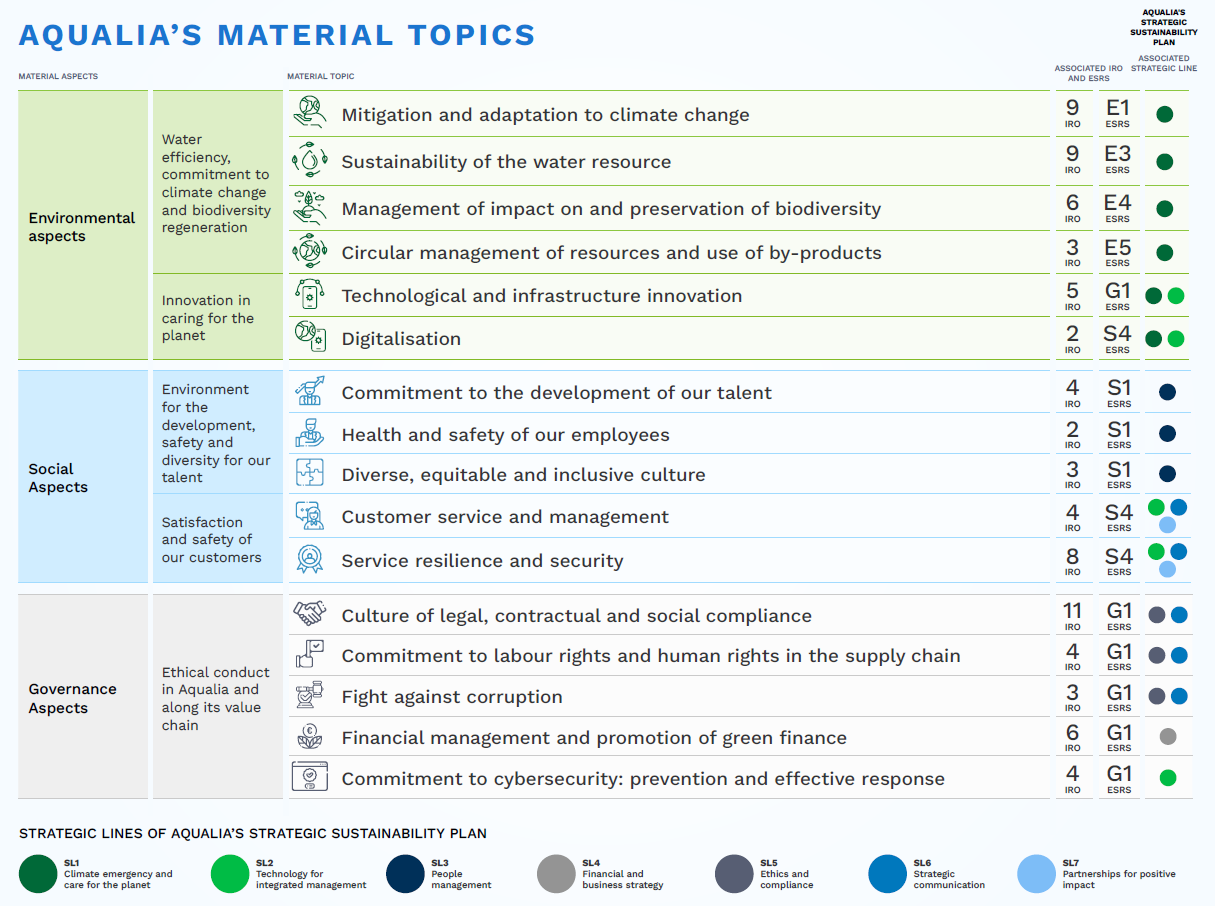
\includegraphics[width=\textwidth]{aqualia_material_topics.png}
\caption[Aqualia's 2025 sixteen material topics]{Aqualia's sixteen material topics as disclosed in the 2025 Double Materiality Review, grouped by environmental (E1--E5), social (S1, S4 plus AQ-tagged topics), and governance (G1 plus AQ-tagged topics) aspects. Source: Aqualia~\cite{aqualiaDMReview2025}.}
\label{fig:aqualiatopics}
\end{figure}

\subsubsection{Three blind spots in Aqualia's 2025 framing}

\begin{enumerate}
\item \signalword{Digitalisation.} Aqualia assigns digitalisation two IROs out of 83, the lowest count among the benchmarked peers. Veolia (AquaCIS), Suez (Aquadvanced), and Global Omnium (GoAigua) each treat digital platforms as a core strategic pillar. The EU Water Resilience Strategy~\cite{waterResilience2025} names digitalisation as Action Area 3 of 5.

\item \signalword{ESRS S3 affected communities.} Aqualia folds community-specific impacts into ESRS~S4 consumer disclosures. Every peer discloses S3 separately. ESRS~S3 explicitly treats communities as distinct from consumers.

\item \signalword{E5 circular economy.} Aqualia's E5 topic carries only three IROs. Veolia and Suez publish quantitative by-product valorisation pipelines; the UWWTD recast~\cite{uwwtd2024} and RD~1985/2024~\cite{rd1985} pull E5 to the regulatory foreground.
\end{enumerate}

\subsubsection{Three differentiators}

First, \signalword{green finance} as a standalone material topic, ahead of peers. Second, \signalword{explicit integration of the double materiality framework with the Corporate Risk Map}, with named Executive Committee owners per risk code. Third, \signalword{TNFD integration alongside CSRD}, an unusual depth among Spanish peers.

\section{Final short-list}

We combine one sector-core pillar with one blind-spot and one differentiator in each topic:

\begin{enumerate}
\item \textbf{T1 Water Resilience \& Equitable Access} (sector-core + S3 restoration). Bundles Aqualia's E1 (9~IROs), E3 (9~IROs), and S4 Service Resilience (8~IROs), with ESRS~S3 restored to surface the Colombia finding. Absorbs 26$+$~IROs.

\item \textbf{T2 Digital \& Cyber Infrastructure} (blind spot). Bundles Technological Innovation (5~IROs), Digitalisation (2~IROs), and Cybersecurity (4~IROs). Absorbs 11~IROs. Our Monte Carlo repositions this cluster into the Target Zone.

\item \textbf{T3 Green Finance \& Integrity} (differentiator amplification). Bundles the G1 cluster (Compliance Culture, 11~IROs; Fight against Corruption, 3; Labour Rights \& Human Rights in Supply Chain, 4) with Financial Management \& Green Finance (6~IROs). Absorbs 24~IROs.
\end{enumerate}

\signalword{Cumulative coverage:} 61 of 83 IROs (73~percent) in Aqualia's 2025 review are absorbed into these three topics; no high-density topic is orphaned.

\begin{callout}
\textbf{Why three, not four or five.} We considered a four-topic shortlist adding either E5 Circular Economy or S1 Workforce Safety. Both sat below our Target Zone on the Monte Carlo scoring, and neither added materially to uncovered IRO mass. A deliberate reduction to three forces real prioritisation across a four-year horizon.
\end{callout}

%% ==========================================================
\chapter{Impact Materiality Assessment}
\label{chap:impact}

\section{Value-chain overlay}

Impacts are assessed along Aqualia's end-to-end water cycle. Upstream impacts (supply-chain human rights, equipment extraction footprint, procurement energy) are attributed to T3 and T2. Own-operations impacts (water abstraction, wastewater-treatment-plant emissions, chemical use, workforce safety, digital-service continuity) are dominated by T1 and T2. Downstream impacts (customer safety, community access to water, biodiversity discharge effects, agricultural reuse) fall primarily within T1 and its restored S3 dimension.

\section{T1 --- Water Resilience and Equitable Access}

Impact materiality for T1 is driven by current, high-severity impacts affecting high-salience stakeholders. Aqualia's own operational risks O1 (deficient supplied-water quality/quantity), O2 (discharge quality impacting ecosystems), O3 (crisis continuity), and O5 (inadequate climate adaptation) are all catalogued HIGH in the Corporate Risk Map. The World Economic Forum's Global Risks Report 2025--2026~\cite{wef2025} ranks five of the top ten long-term risks as water-related and projects global water demand to exceed supply by 40~percent by 2030.

The restored S3 dimension introduces what we term the \emph{Colombia finding}: Aqualia's 2024 customer-satisfaction survey, in a sample of more than seven thousand respondents, reports satisfaction ranging 86--98~percent across Spain, Portugal, France, Italy, the Czech Republic, and institutional markets~\cite{aqualiaSR2024}. In Colombia, satisfaction stands at \signalword{33~percent}. A 55-point spread sits inside a single group-level metric. Under ESRS~S3, which specifically concerns affected communities rather than end-users, the same data carries different remediation and concession-renewal implications.

The context for elevating water-resilience to the highest-severity topic is not limited to Aqualia's own data. Figure~\ref{fig:wefrisks} reproduces the World Economic Forum's \emph{Global Risks 2025--2026} severity ranking. Five of the top ten ten-year risks are water- or ecosystem-related. This independent external signal corroborates T1's position in our matrix.

\begin{figure}[htbp]
\centering
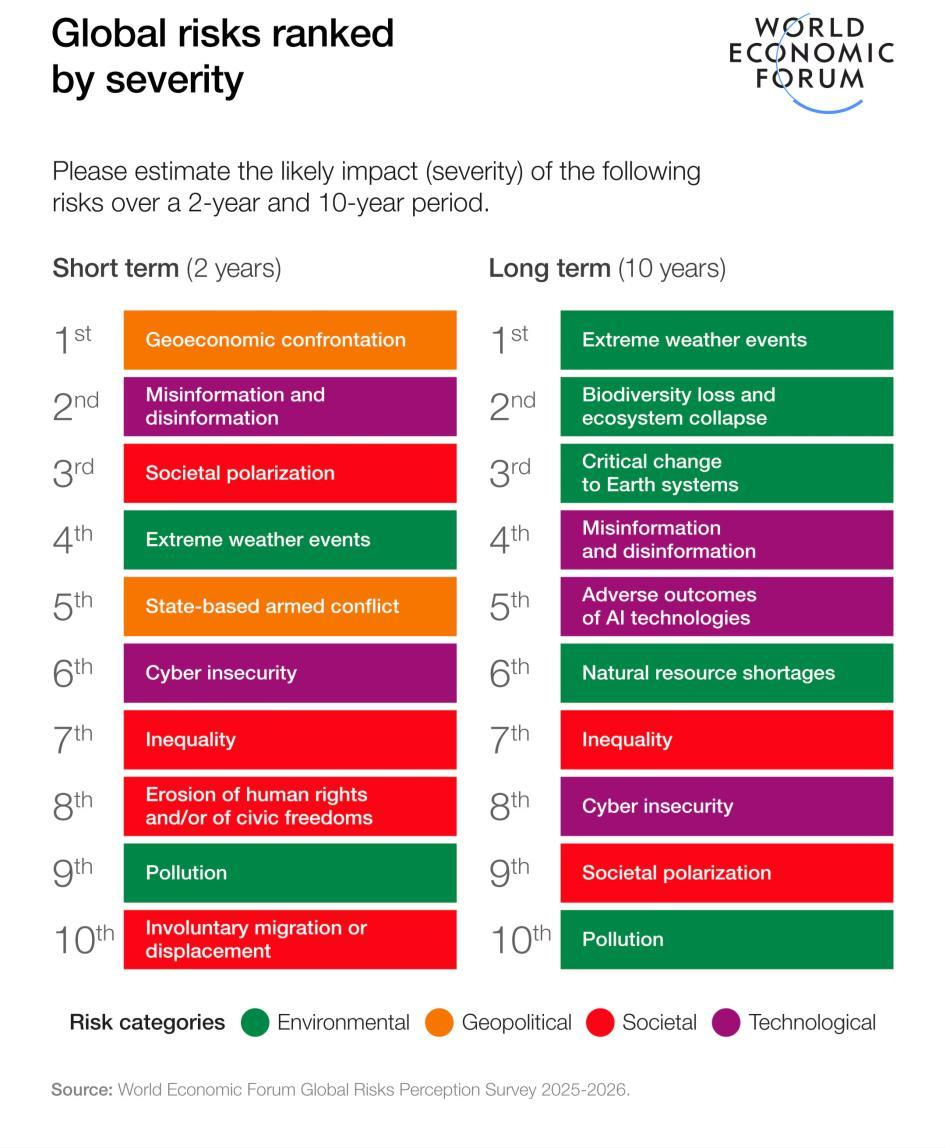
\includegraphics[width=0.78\textwidth]{wef_global_risks.png}
\caption[WEF Global Risks 2025--2026]{Global risks ranked by severity, 2-year and 10-year horizons. Extreme weather, biodiversity loss, critical change to Earth systems, natural resource shortages, and pollution are five of the top ten ten-year risks. Source: WEF Global Risks Report~\cite{wef2025}.}
\label{fig:wefrisks}
\end{figure}

\begin{insight}
\textbf{Monte Carlo mean Impact Severity for T1: 3.98}, with a 90\% interval of $[3.87, 4.09]$. Solidly in the Target Zone; further than any other topic from the 2.5 threshold on either axis.
\end{insight}

\section{T2 --- Digital and Cyber Infrastructure}

Impact materiality for T2 is driven by three operational risks Aqualia itself rates HIGH: O8 (poor digital deployment), O9 (deficient cyber response plan), and O10 (customer-data management), despite the topic carrying only two IROs in the 2025 matrix. The stakeholder-salience weighting amplifies the signal: Customers (0.120), Public Authorities (0.120), Employees (0.120), and Investors (0.080) are all materially affected by digital and cyber performance. Peer comparators demonstrate that digital capability has direct impact materiality on service continuity and data privacy: the Thames Water 2023 cyber-incident disclosure and the Severn Trent 2024 operational-technology/information-technology exposure update both quantify service-continuity impacts on millions of users.

\begin{insight}
\textbf{Monte Carlo mean Impact Severity for T2: 3.08}, with a 90\% interval of $[2.93, 3.24]$. Inside the Target Zone but closer to the threshold than T1.
\end{insight}

\section{T3 --- Green Finance and Integrity}

Impact materiality for T3 is governance-heavy. The Compliance cluster (eleven IROs) covers CSRD reporting obligations, contract compliance with Public Administrations and private principals, Corporate Compliance Management System alignment, and tax compliance, each with a named owner in Aqualia's Risk List. Labour rights and human rights in the supply chain (four IROs) introduce workforce impacts upstream. Green finance as a standalone topic (six IROs) creates a positive-impact channel via capital-markets signalling to investors and rating agencies.

\begin{insight}
\textbf{Monte Carlo mean Impact Severity for T3: 3.24}, with a 90\% interval of $[3.08, 3.41]$.
\end{insight}

\section{The Colombia outlier}

We treat the Colombia finding as a standalone narrative thread. The spread between Colombia (33~percent) and the next-lowest market (Portugal, 65~percent) is 32~points; the spread to Italy (67~percent) is 34~points; to Spain (88~percent) is 55~points. Aqualia's 2025 review does not discuss Colombia specifically in the S4 topic; the framing treats satisfaction as a group-level customer-experience measure. Under ESRS~S3, which specifically concerns affected communities rather than end-users, a 33~percent satisfaction market with ongoing supply reliability issues represents material impact on affected communities.

Our recommendation is to re-surface ESRS~S3 as its own disclosure rather than as a subset of S4, starting with the 2027 reporting cycle. The operational corollary is a Colombia-specific community action plan with named Executive Committee ownership and a quantified satisfaction-recovery KPI. Both are developed in Chapter~\ref{chap:roadmap}.

%% ==========================================================
\chapter{Financial Materiality Assessment}
\label{chap:financial}

\section{Per-topic financial decomposition}
\label{sec:perfin}

Each topic decomposes into five financial channels: revenue at risk, revenue upside, OPEX impact, CAPEX needs, and contingent liabilities. For each channel we estimate a triangular distribution (low/base/high) anchored to Aqualia's public financial scale, peer disclosures, and regulatory cost factors. The full assumption log (A01--A17) is in Appendix~B.

\subsubsection{T1}

Revenue at risk of \euro{}25--110~M from concession loss and tariff pressure in water-stressed basins (A03); revenue upside of \euro{}15--75~M from the reuse market under RD~1985/2024 and nature credits (A04); OPEX impact of \euro{}8--32~M per year under UWWTD recast and chemical cost inflation (A05); CAPEX needs of \euro{}220--520~M cumulative 2027--2030 across desalination, reuse, leak reduction, and WWTP energy-neutrality (A06); contingent liabilities of \euro{}10--65~M from Water Framework Directive and service-continuity fines (A07).

\subsubsection{T2}

Revenue at risk of \euro{}12--80~M from cyber-incident service interruption and GDPR/NIS2 fines (A08); revenue upside of \euro{}8--45~M from tender win-rate uplift on digital differentiation (A09); OPEX impact of \euro{}4--14~M per year on cyber and IT above baseline (A10); CAPEX of \euro{}45--130~M cumulative on digital-twin rollout and OT/IT segmentation (A11); contingent liabilities of \euro{}5--56~M from NIS2 and GDPR maximum fines (A12).

\subsubsection{T3}

Revenue at risk of \euro{}8--50~M from ESG-laggard cost-of-capital spread and financing-window loss (A13); revenue upside of \euro{}6--28~M from green-bond coupon savings (A14); cost-of-capital saving of \euro{}4--24~M per year over the refinancing cycle (A15); CAPEX of \euro{}8--35~M cumulative on compliance systems (A16); contingent liabilities of \euro{}3--35~M from CSDDD civil-liability and Omnibus-I interactions (A17).

\section{Five-dimension mapping to the brief}

The Datathon brief (\S 3) requires financial materiality to be assessed against \emph{revenues, costs, assets, liabilities, and enterprise value}. Each topic's principal R\&O channels tag explicitly to these five dimensions as shown in Table~\ref{tab:fivedim}.

\begin{table}[h]
\caption{Five-dimension financial mapping by topic}
\label{tab:fivedim}
\centering
\small
\renewcommand{\arraystretch}{1.35}
\begin{tabular}{@{}p{1.3cm}p{2.9cm}p{2.6cm}p{2.8cm}p{2.4cm}p{2.5cm}@{}}
\toprule
\textbf{Topic} & \textbf{Revenues} & \textbf{Costs} & \textbf{Assets} & \textbf{Liabilities} & \textbf{Ent.\ value} \\
\midrule
\textbf{T1} & \euro{}25--110~M at risk; \euro{}15--75~M upside & \euro{}8--32~M/yr OPEX & \euro{}220--520~M CAPEX; stranded-asset risk & \euro{}10--65~M contingent (WFD, CSDDD) & Concession-renewal multiple discount \\[2pt]
\textbf{T2} & \euro{}8--45~M tender uplift; interrupt.\ risk & \euro{}4--14~M/yr cyber \& digital OPEX & \euro{}45--130~M CAPEX on twin \& OT/IT & \euro{}5--56~M GDPR/NIS2 fines & Tech-differentiation multiple uplift \\[2pt]
\textbf{T3} & --- & \euro{}8~M/yr cost-of-capital saving (\euro{}31~M PV) & --- & Bond $\leq$ vanilla; CSDDD \euro{}3--35~M & ESG-rating re-rating \\
\bottomrule
\end{tabular}
\end{table}

\section{The \euro{}18~M/yr headline --- full derivation}

Aggregating the net recurring annual financial materiality (revenue at risk minus revenue upside minus cost-of-capital saving; CAPEX excluded because it is investment, not recurring materiality) yields:

\begin{center}
\small
\renewcommand{\arraystretch}{1.3}
\begin{tabular}{@{}p{1.5cm}p{3.3cm}p{8.5cm}@{}}
\toprule
\textbf{Topic} & \textbf{Net recurring} & \textbf{Composition} \\
\midrule
T1 & $-$\euro{}15~M/yr & $-$55 revenue at risk $+$ 40 reuse upside \\
T2 & $-$\euro{}8~M/yr & $-$30 revenue at risk $+$ 22 tender uplift \\
T3 & $+$\euro{}5~M/yr & $-$22 compliance drag $+$ 15 rating premium $+$ 12 CoC saving \\
\midrule
\textbf{Total} & \signalword{$-$\euro{}18~M/yr} & Net drag the current framework under-weights \\
\bottomrule
\end{tabular}
\end{center}

This \euro{}18~million per year figure is recurring, not one-off, and explicitly excludes the \euro{}440~million cumulative 2027--2030 CAPEX. Under $\pm 20$~percent revenue-anchor sensitivity (A01), the headline scales to $-\euro{}14$~M per year at the low anchor or $-\euro{}22$~M per year at the high anchor. The sign and the conclusion are stable in both directions.

\section{Aqueduct water-stress overlay}

The T1 financial case depends critically on the geographic exposure of Aqualia's concession base to water stress. Using WRI Aqueduct~4.0 baseline water-stress categories overlaid on Aqualia's declared service geography, we estimate that 45~percent of Aqualia's revenue base operates in basins classified High or Extremely High water stress today (Segura, Guadalquivir, Po, Sicily, Algarve, Languedoc). Under a BAU-2030 climate scenario (SSP3/RCP 7.0), that share nearly doubles to 79~percent. This is the principal driver of assumption A03 and the main sensitivity lever in the tornado analysis. Figure~\ref{fig:aqueduct} shows the basin-level decomposition.

\begin{figure}[htbp]
\centering
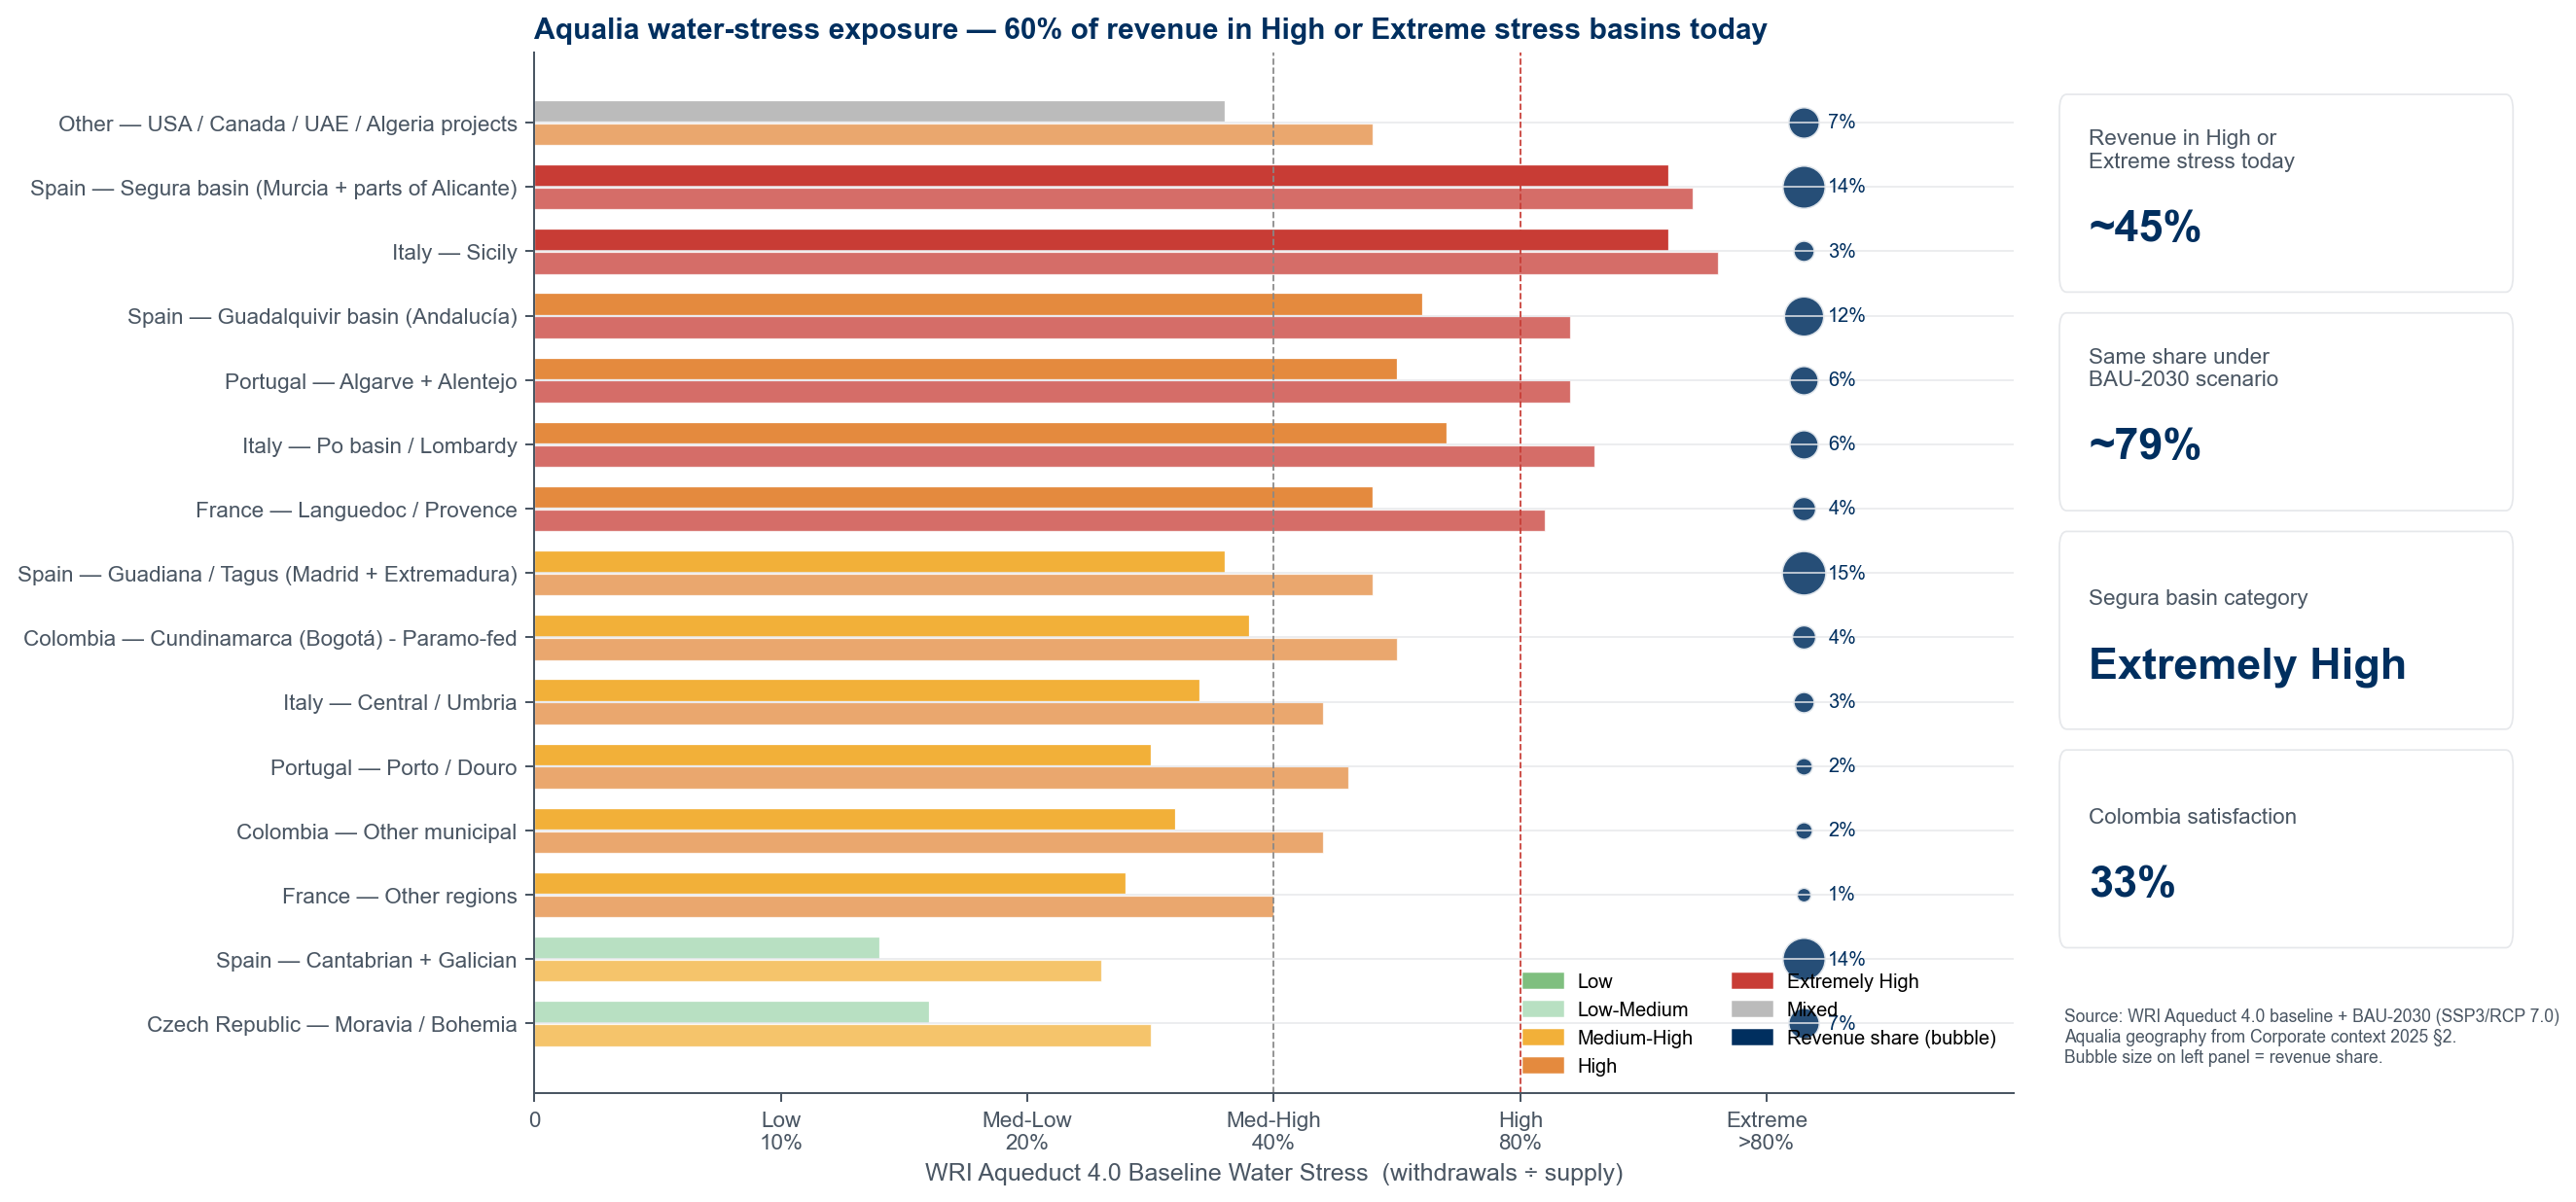
\includegraphics[width=0.95\textwidth]{aqueduct_exposure.png}
\caption[WRI Aqueduct 4.0 baseline water-stress exposure for Aqualia concessions]{Baseline water stress (WRI Aqueduct 4.0) overlaid on Aqualia's service geography, per basin. Left bars: 2024 baseline. Right bars: 2030 under SSP3/RCP 7.0. 45\% of revenue sits in High or Extremely High stress basins today; 79\% by 2030.}
\label{fig:aqueduct}
\end{figure}

\section{Real Options --- desalination versus water reuse}

Within T1's CAPEX envelope, the largest single capital-allocation decision is desalination capacity expansion versus water-reuse infrastructure. Under indicative parameters (desalination PV \euro{}145~M, $\sigma$~28\%; water-reuse PV \euro{}135~M, $\sigma$~38\%; three-year deferral window; 3\% risk-free rate), a Black--Scholes-style real-options calculation yields:

\begin{center}
\small
\begin{tabular}{lccc}
\toprule
\textbf{Option} & \textbf{Immediate NPV} & \textbf{Deferral option value} & \textbf{Total value} \\
\midrule
Desalination & \euro{}25~M & \euro{}18~M & \euro{}43~M \\
Water reuse & \euro{}40~M & \euro{}29~M & \textbf{\euro{}69~M} \\
\bottomrule
\end{tabular}
\end{center}

Water reuse dominates on both immediate NPV and optionality because reuse volumes scale more flexibly with realised demand. Final numbers require Aqualia's asset-level cost of capital and tariff structure; the exhibit is positioned as illustrative (see Limitations, Chapter~\ref{chap:limits}).

\section{The \euro{}500~M green bond proposal}

The 2027--2030 CAPEX implied by Aqualia's Risk Map and our three topics totals \euro{}440~M base case (\euro{}285--685~M under low/high assumptions). We propose funding the programme via a \signalword{\euro{}500~million EU-Taxonomy-aligned green / sustainability-linked bond programme}, issued in four tranches: \euro{}150~M in 2027, \euro{}150~M in 2028, \euro{}120~M in 2029, \euro{}80~M in 2030. Structural choices (use-of-proceeds versus sustainability-linked; coupon step-up KPIs tied to NRW reduction and water-reuse ratio) are detailed in the roadmap (Chapter~\ref{chap:roadmap}).

At a 25~basis-point coupon spread --- the 2024--2025 level for investment-grade Euro water-utility green issuance per Climate Bonds Initiative data~\cite{cbi2024} --- the programme delivers \signalword{\euro{}31~M of present-value interest savings} over the bond life (ten-year tenor, 4.00\% vanilla versus 3.75\% green coupon, 8\% discount rate). The calculation is the discounted annuity of the coupon saving: $500 \times 25~\text{bp} \times A(10, 8\%) \approx$ \euro{}8.4~M nominal annual saving, yielding \euro{}31.1~M PV. The estimate is conservative: the spread regularly exceeds 25~bp in Iberian and Italian issuance, where Aqualia's concession base concentrates.

%% ==========================================================
\chapter{The Double Materiality Matrix}
\label{chap:matrix}

\section{Matrix structure}

The matrix (Figure~\ref{fig:matrix}) plots Impact Severity (y-axis, inside-out) against Financial Severity (x-axis, outside-in), each on a 1--5 scale. The Target Zone is the top-right quadrant with both axes $\geq 2.5$. Each topic appears as a 90\% confidence ellipse derived from 10{,}000 Monte Carlo draws. The ellipse centroid marks the topic's mean position. Topics with ellipses entirely inside the Target Zone are classified \emph{robust material}; topics with ellipses straddling threshold lines are classified \emph{conditionally material}.

\begin{figure}[htbp]
\centering
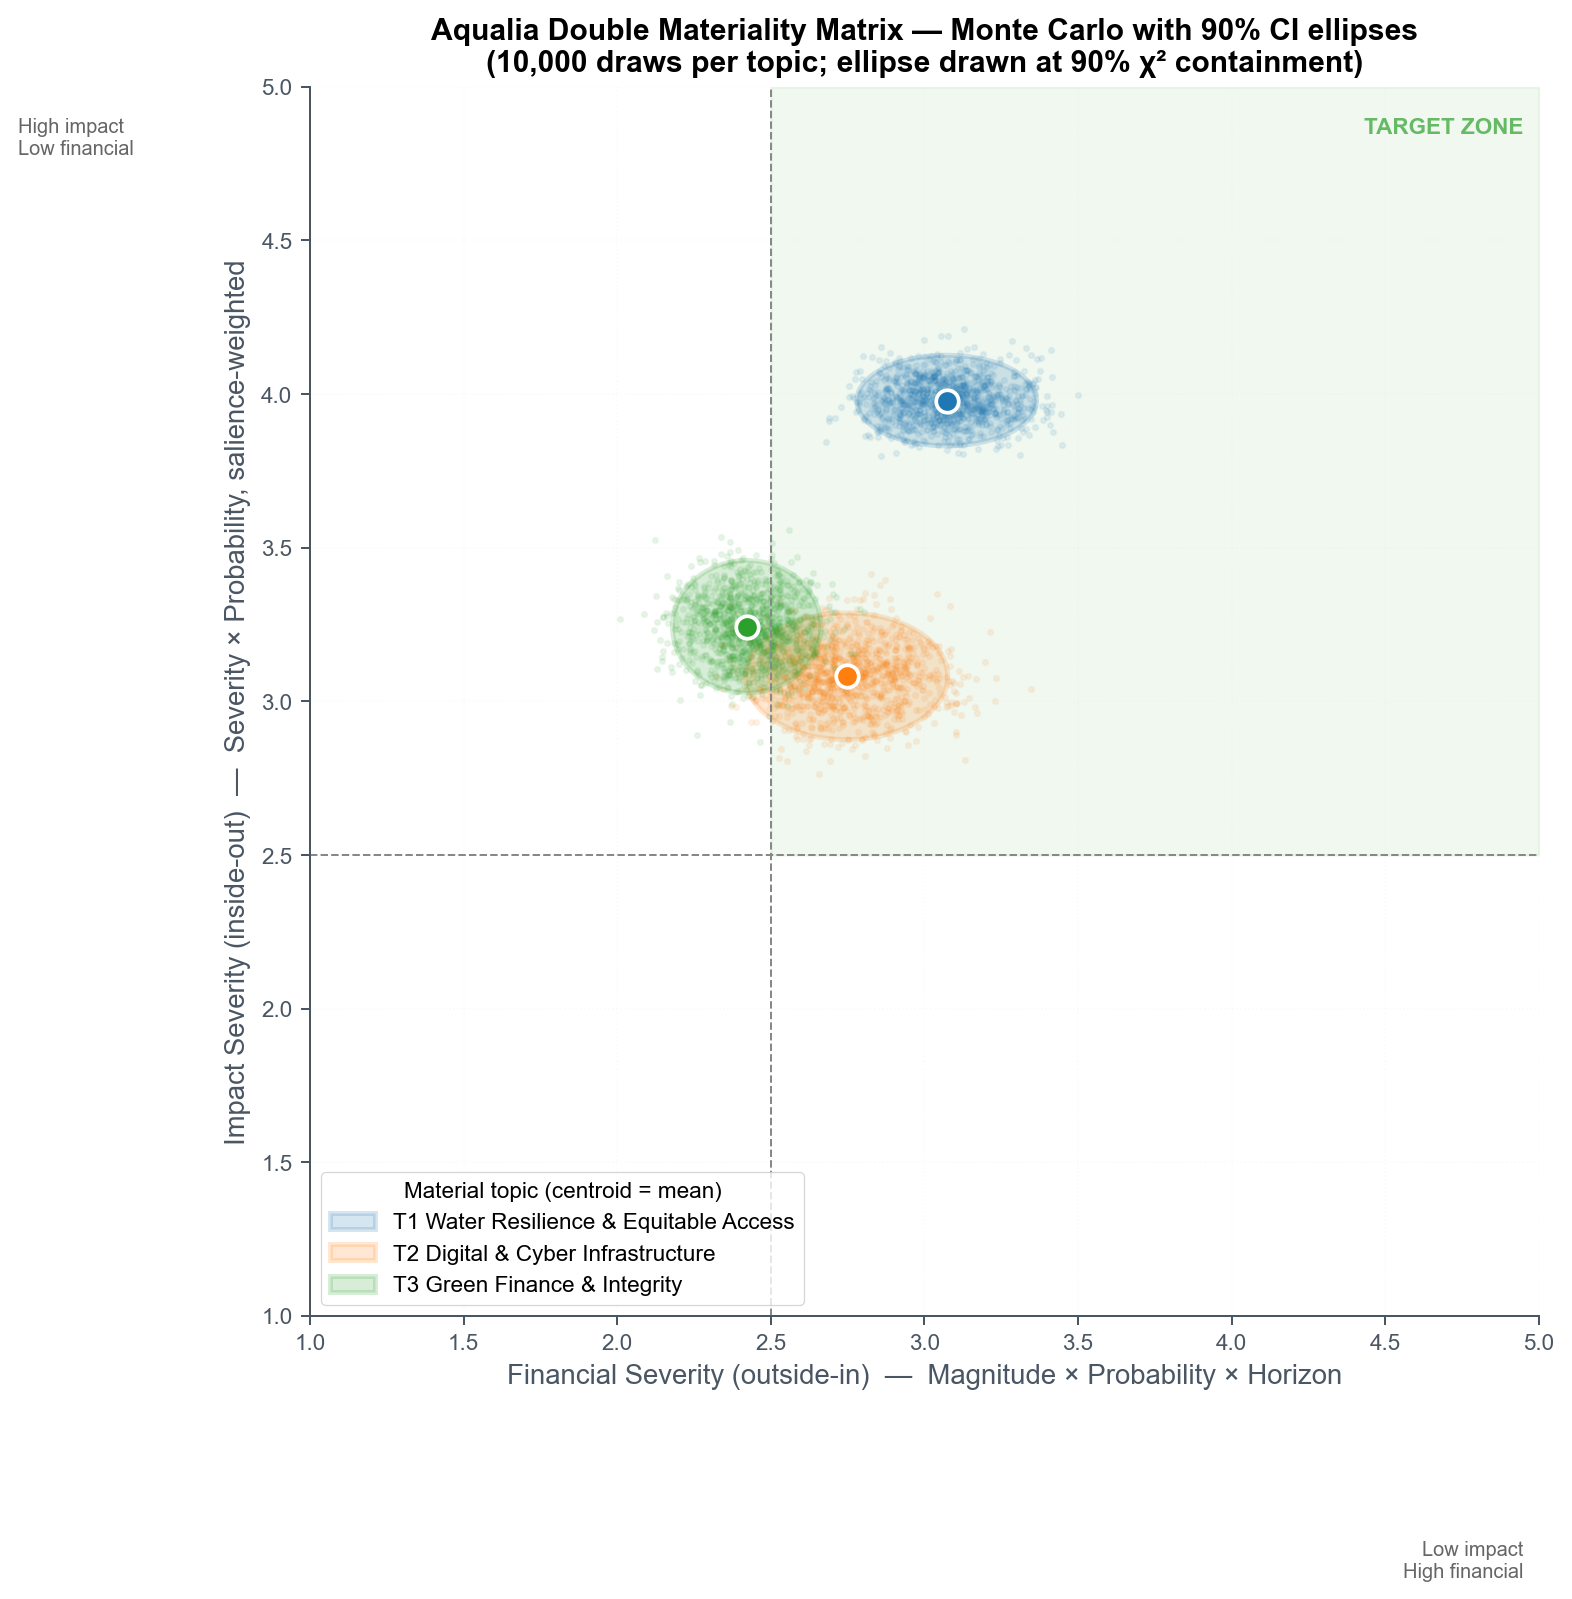
\includegraphics[width=0.85\textwidth]{matrix_mc.png}
\caption{Double materiality matrix for Aqualia's three short-listed topics. Each ellipse encloses 90\% of 10{,}000 Monte Carlo outcomes. The Target Zone (shaded) is defined as Impact Severity~$\geq 2.5$ and Financial Severity~$\geq 2.5$.}
\label{fig:matrix}
\end{figure}

\section{Per-topic positioning}

\subsubsection{T1 centroid (3.07, 3.98)}

Ellipse wholly inside the Target Zone and bounded well away from both threshold lines. T1 is robust material under every test we ran.

\subsubsection{T2 centroid (2.75, 3.08)}

Ellipse lies inside the Target Zone; the financial-axis fifth percentile sits at 2.50, right on the boundary. That fact confirms T2's Target Zone membership is directly attributable to our repositioning of the blind-spot cluster. Under Aqualia's original qualitative framework (two IROs on Digitalisation alone), T2 would not be material; under our methodology it is.

\subsubsection{T3 centroid (2.42, 3.24)}

Ellipse centroid lies 0.08 below the financial threshold, with $p_{95}$ at 2.61 and $p_5$ at 2.24. T3 is conditionally material: Target Zone on impact, borderline on finance. This is the most informative methodological outcome of the study: it distinguishes between solidly and conditionally material topics where a qualitative framework would paint both the same colour.

\section{Sensitivity drivers}
\label{sec:sensitivity}

For each topic, the top six inputs by absolute swing are:

\begin{description}
\item[T1] R-stress-revenue magnitude (financial); E1-adaptation probability (impact); O-reuse-market magnitude (financial); R-CAPEX-UWWTD magnitude (financial); E3-quality scale (impact); R-fines-WFD magnitude (financial). The water-stress revenue assumption (A03) and the reuse-market sizing (A04) dominate financial position; the probability of climate adaptation dominates impact. Both are grounded in Aqueduct and RD~1985/2024 and should be tightened in a production-grade refresh.

\item[T2] Tech-pace probability (impact); O-tender-uplift magnitude (financial); R-digital-CAPEX magnitude (financial); Dig-data-governance probability (impact); Dig-adoption scale (impact); Tech-pace scale (impact). The key question is how much digital differentiation translates into tender-win uplift. An expert call is the single highest-return-on-investment validation data-point.

\item[T3] Compl-CSDDD probability (impact); Green-fin-access probability (impact); Compl-CSRD scale (impact); O-green-bond-premium magnitude (financial); Green-fin-access scale (impact); O-CoC-saving magnitude (financial). T3's position is a bet on regulatory enforcement pace plus cost-of-capital spread, both observable and both directly targeted by the \euro{}500~M bond programme.
\end{description}

\begin{figure}[htbp]
\centering
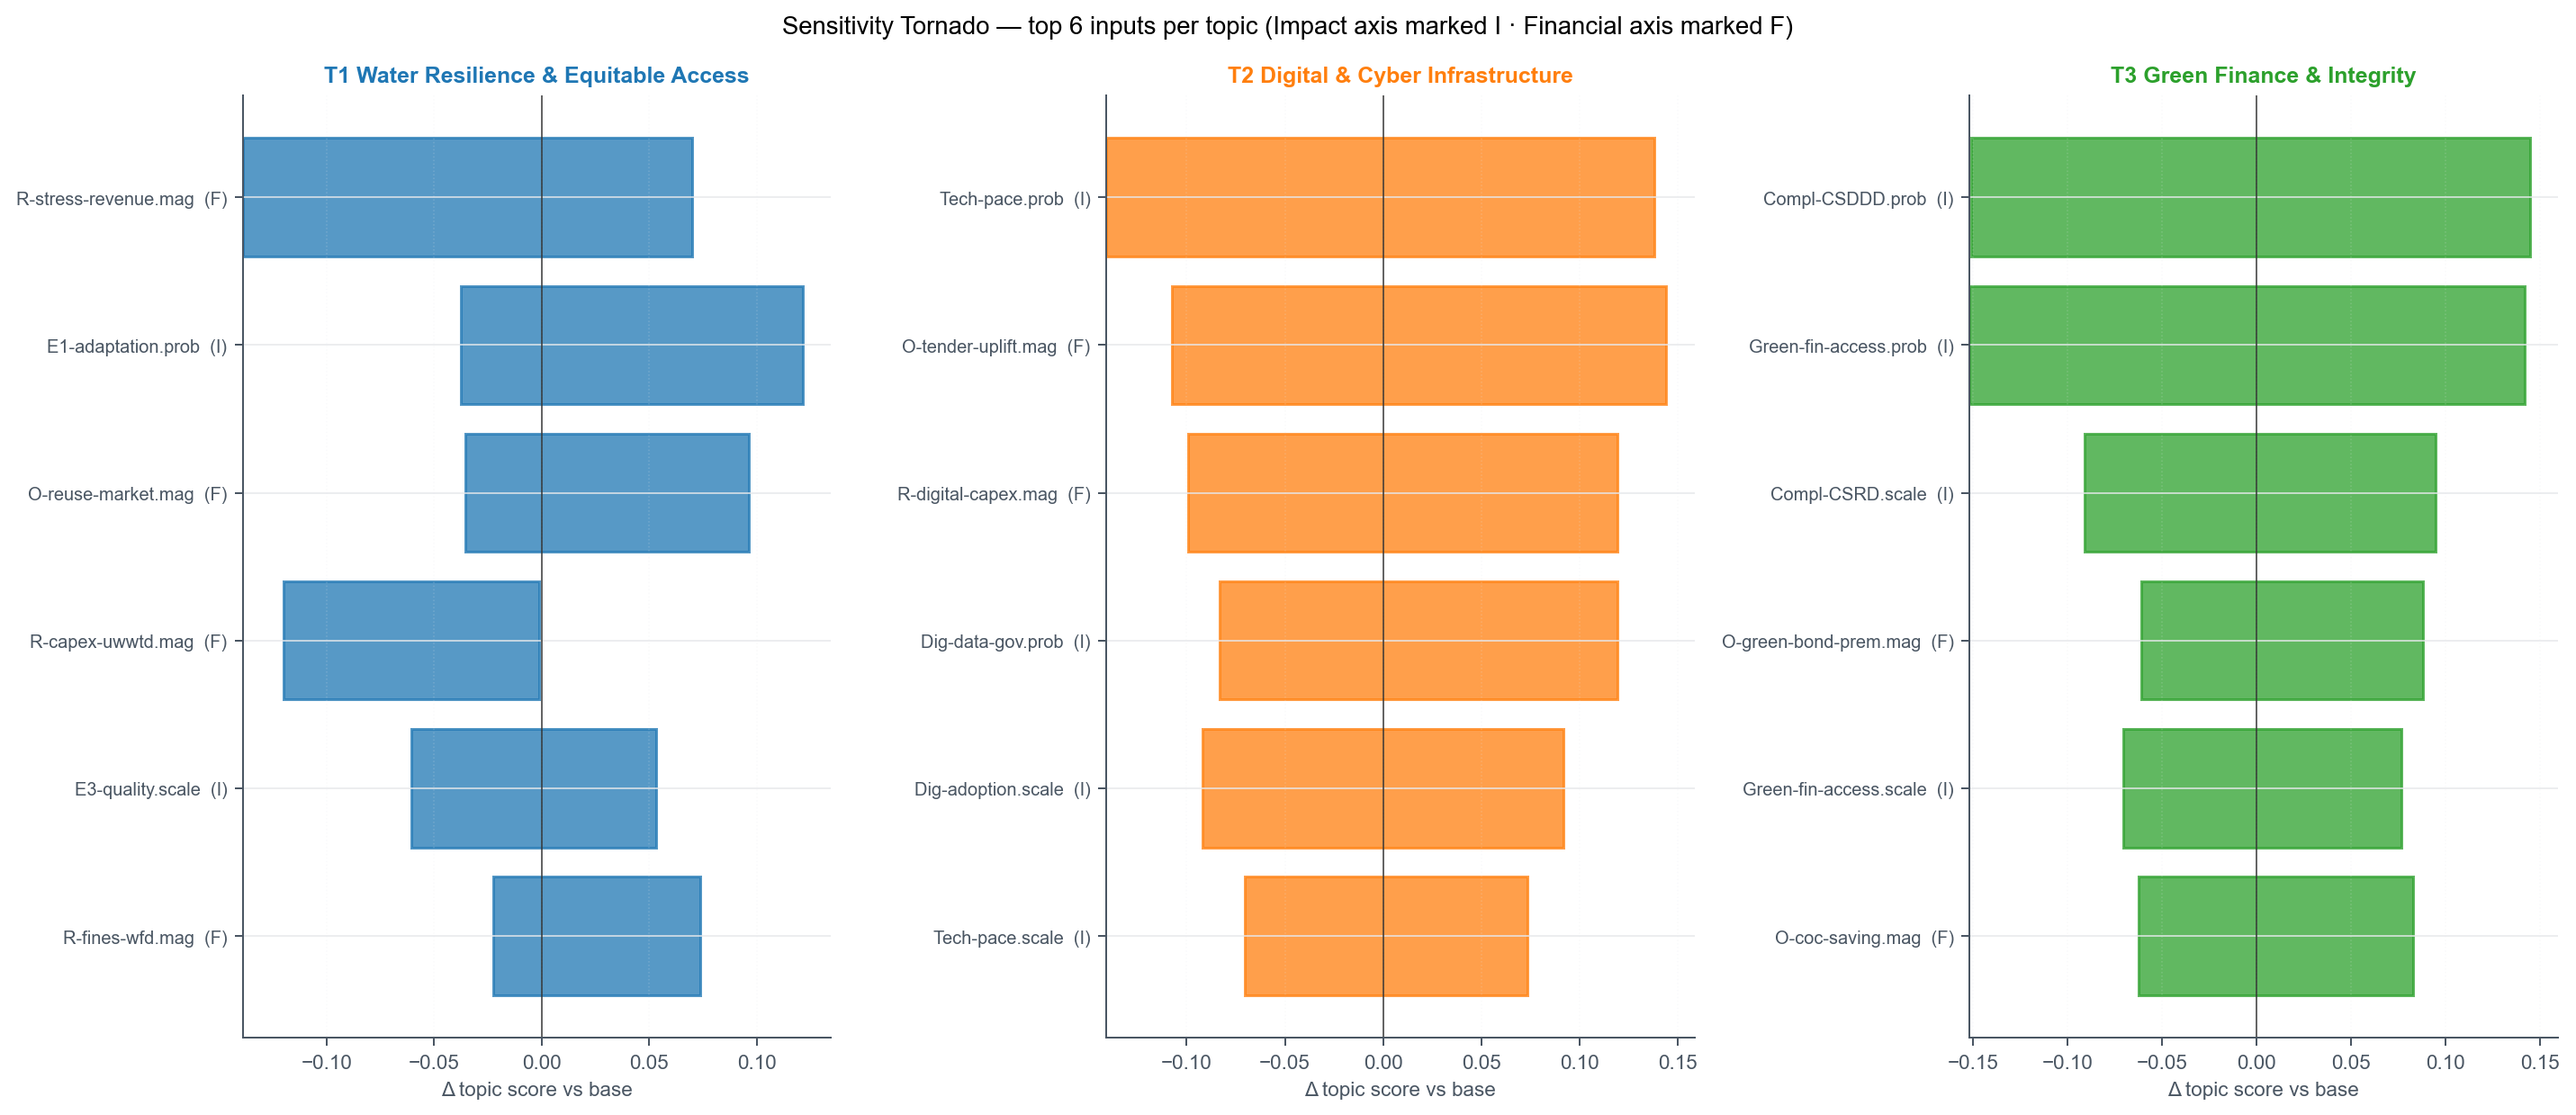
\includegraphics[width=\textwidth]{matrix_tornado.png}
\caption[Monte Carlo sensitivity tornado, per topic]{Sensitivity tornado per topic from the Monte Carlo pipeline. Horizontal bars show the change in topic-centroid position when each input is perturbed at the top and bottom of its plausible range, holding others at base. Top six drivers per topic shown.}
\label{fig:tornado}
\end{figure}

\section{Robustness across weighting schemes}

Under four alternate stakeholder-weighting schemes (Equal, Regulator-heavy, Community-first, Investor-first), no topic flips Target-Zone status. T1 remains in; T2 remains in; T3 remains borderline. The stability is a direct consequence of top-$k$ aggregation: the most material subset of IROs and R\&Os drives position, and that subset is insensitive to modest re-weighting.

\section{ESRS disclosure coverage context}

Figure~\ref{fig:heatmap} summarises the ESRS disclosure-gap heatmap generated from the bilingual TF--IDF pipeline. Aqualia's overall coverage across seventy-five canonical datapoints is 35~percent (Strong + Partial bands combined), against a directional peer-benchmark average of approximately 63~percent. The ESRS~S3 row is the most dark-red row in the heatmap, supporting the methodological case for S3 restoration developed in Chapter~\ref{chap:impact}.

\begin{figure}[htbp]
\centering
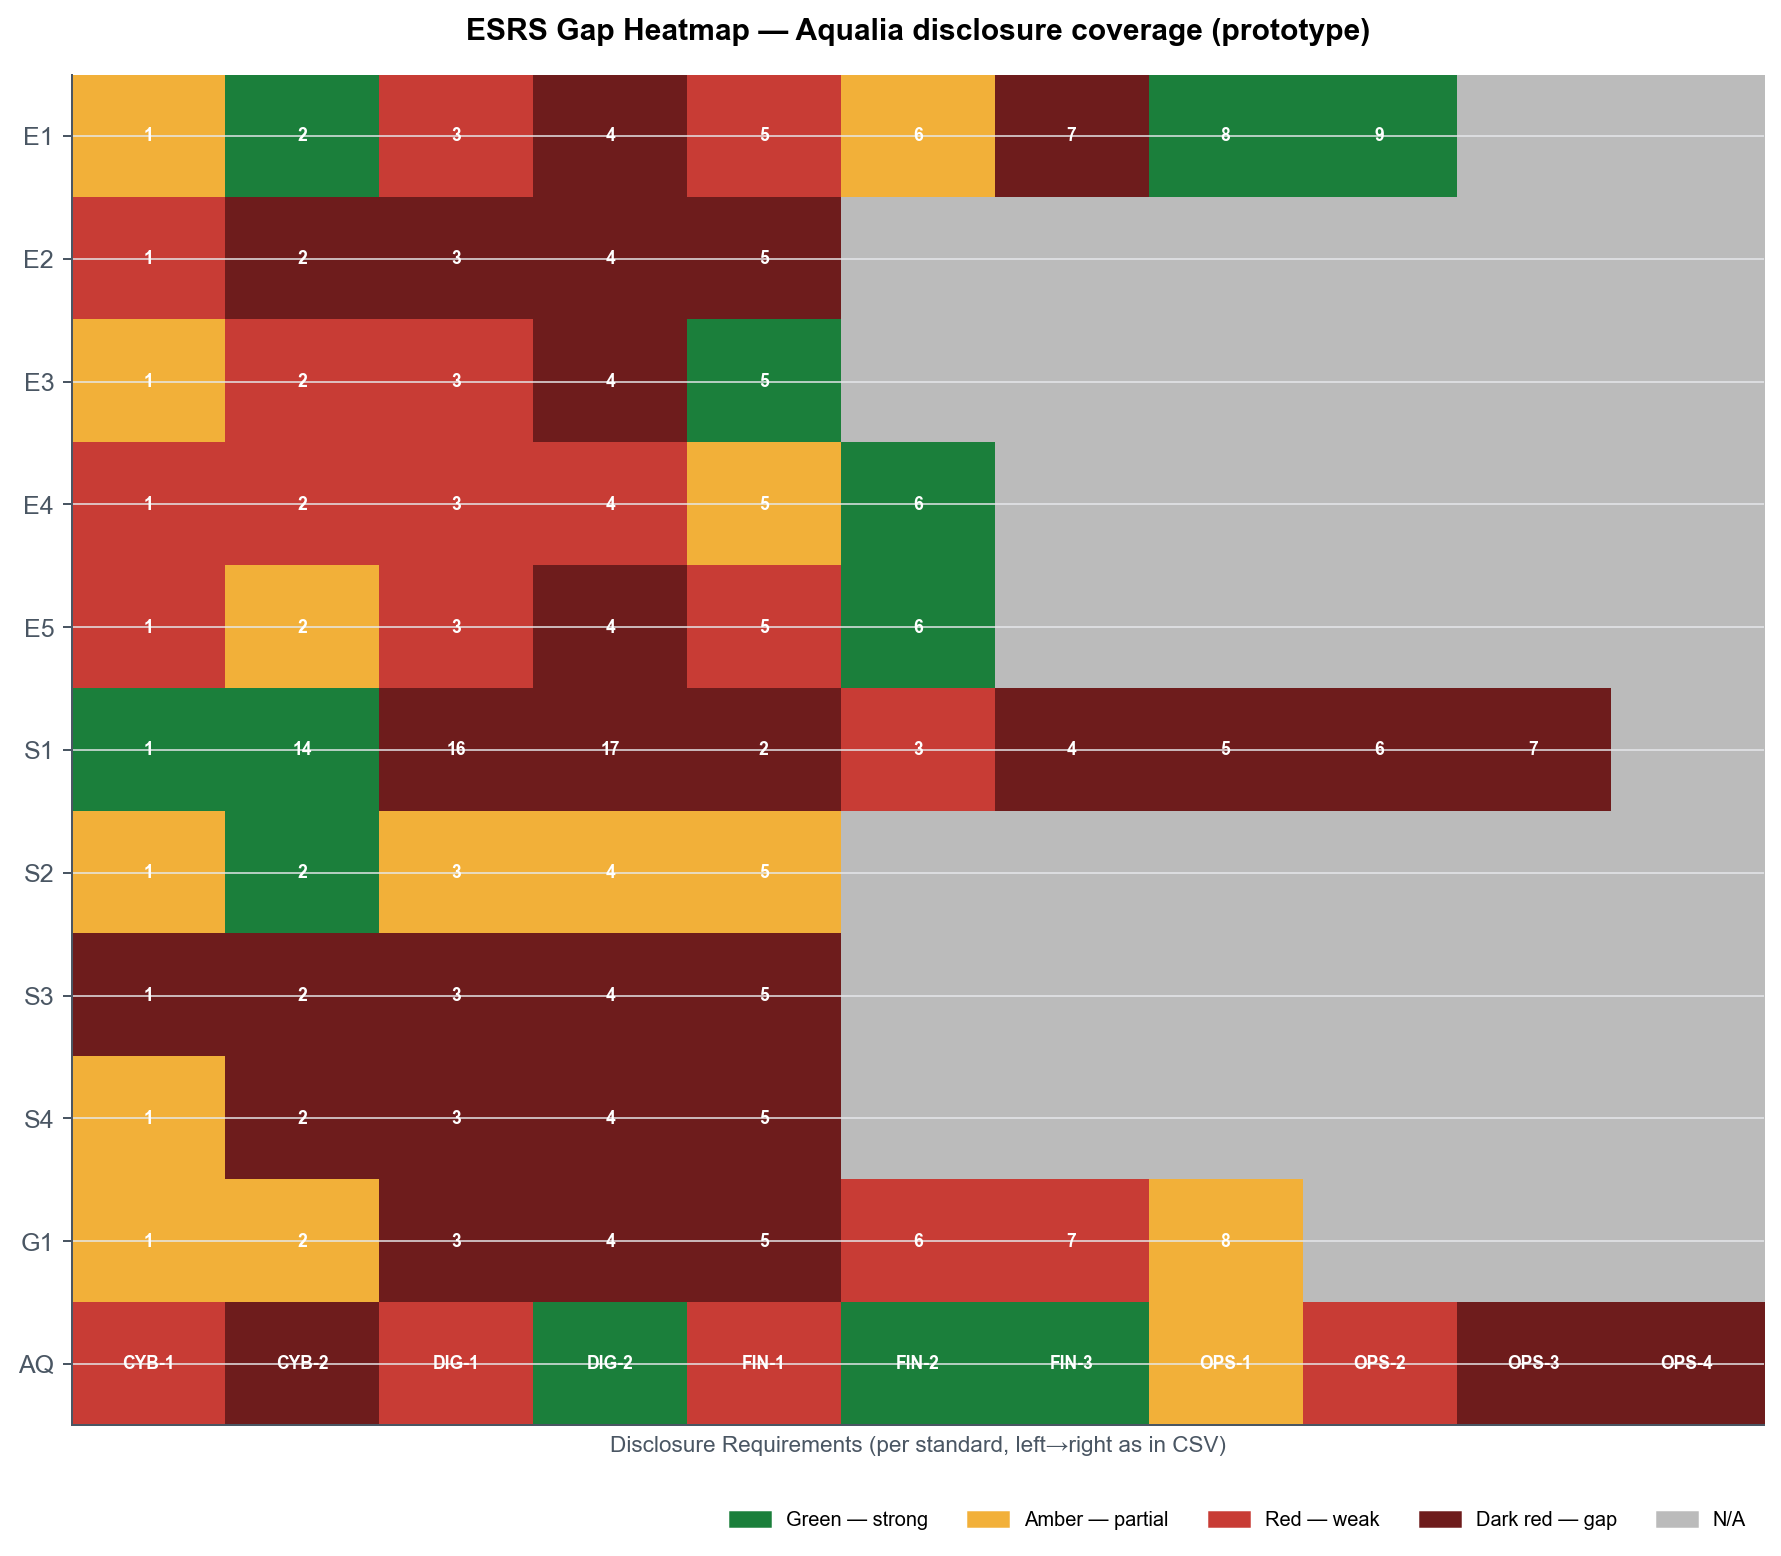
\includegraphics[width=0.95\textwidth]{esrs_gap_heatmap.png}
\caption{ESRS disclosure-gap heatmap. Seventy-five canonical ESRS datapoints (rows) against Aqualia's 2022--2025 corpus coverage bands (colour). The ESRS~S3 row (affected communities) shows structural gaps that our first recommendation addresses.}
\label{fig:heatmap}
\end{figure}

%% ==========================================================
\chapter{Strategic Sustainability Roadmap 2027--2030}
\label{chap:roadmap}

\section{Owned. Measurable. Aligned.}

Every recommendation is assigned to a named Executive Committee role using Aqualia's own Risk Map owners, and pinned to a quantitative KPI. The roadmap is structured as a three-topic by four-year grid.

\subsubsection{T1 --- Water Resilience \& Equitable Access}

\begin{itemize}
\item \textbf{2027.} Restore ESRS~S3 as a standalone disclosure. Commission a Colombia concession review. Owner: Director Spain, Europe/Americas, Africa/Asia. KPI: Colombia satisfaction~$\geq 60\%$ by year-end; S3 disclosure appearing in the 2027 sustainability report.
\item \textbf{2028.} Segura basin water-reuse pilot. Owner: Director Studies \& Operations. KPI: Non-Revenue Water down 3 percentage points in pilot concession; reuse water volume up 15\% versus 2025 baseline.
\item \textbf{2029.} Italy climate-adaptation CAPEX programme; Po basin focus. Owner: Director Spain/EU/Americas/AA. KPI: emissions intensity down 10\% per m$^3$ treated; 100\% ISO~14001:2026 coverage.
\item \textbf{2030.} Full-group reuse~$\geq 25\%$ of treated wastewater; alignment with RD~1985/2024. KPI: reuse ratio~$\geq 25\%$; WFD compliance clean across Iberian concessions.
\end{itemize}

\subsubsection{T2 --- Digital \& Cyber Infrastructure}

\begin{itemize}
\item \textbf{2027.} Digital-twin Phase~1 --- three concessions. Owner: Customer \& IT Management Director. KPI: real-time monitoring coverage~$\geq 80\%$ of treated volume in pilot.
\item \textbf{2028.} OT/IT segmentation and NIS2 readiness assessment. Owner: Customer \& IT Management Director. KPI: NIS2 readiness~$\geq 90\%$ per internal audit.
\item \textbf{2029.} AI demand-prediction and leak-detection rollout beyond pilot. Owner: Director Strategy \& Sustainability Development. KPI: leak-detection response time down 30\%.
\item \textbf{2030.} Cyber-incident mean-time-to-recover (MTTR)~$<~4$~hours under simulated red-team tests; annual cyber investment at approximately 1.0\% of revenue.
\end{itemize}

\subsubsection{T3 --- Green Finance \& Integrity}

\begin{itemize}
\item \textbf{2027.} Issue Tranche~1 of green bond programme (\euro{}150~M). Owner: CFO. KPI: tranche closed at $\leq~20$~bp premium to vanilla comparable; EU-Taxonomy alignment report published.
\item \textbf{2028.} Tranche~2 (\euro{}150~M). Full CSRD report with limited assurance. Owner: CFO and Sustainability Director.
\item \textbf{2029.} Tranche~3 (\euro{}120~M). ISO~14001:2026 certification across all operating regions~\cite{iso14001}.
\item \textbf{2030.} Tranche~4 (\euro{}80~M). Full TCFD and TNFD disclosure with reasonable assurance. KPI: TNFD LEAP coverage $\geq 90\%$ of in-scope concessions.
\end{itemize}

\section{Integration with Aqualia's Strategic Sustainability Plan}

Aqualia's 2024--2026 Strategic Sustainability Plan operates along seven strategic lines. Our roadmap is designed to \emph{extend} that plan into 2027--2030 rather than replace it. T1 extends the Climate Emergency line. T2 extends the Technology-for-Integrated-Management line. T3 extends the Financial \& Business Strategy and Ethics \& Compliance lines. The cross-walk between our twelve quarterly milestones and the seven strategic lines is fully traceable; no recommendation sits outside Aqualia's existing strategic architecture.

\section{Governance and reporting cadence}

We recommend Aqualia's Sustainability Committee adopt a \signalword{semi-annual matrix refresh} using the reproducible Monte Carlo pipeline. Each refresh produces updated confidence ellipses under the latest input assumptions; material shifts in ellipse position across two consecutive refreshes should trigger Executive Committee review. This institutionalises the methodology rather than treating it as a one-off deliverable.

%% ==========================================================
\chapter{Limitations, Reverse Stress Test, and Ethical Framing}
\label{chap:limits}

\section{What this methodology cannot do}

Six honest limitations, each with a remediation path.

\begin{enumerate}
\item \signalword{No external stakeholder consultation in this cycle.} Mirrors Aqualia's own 2025 cycle choice but inherits its consequence. Remediation: the Mitchell--Agle--Wood salience model is a \emph{substitute} for consultation, not a \emph{replacement}. A production-grade version should conduct at least one round of external interviews per stakeholder group over the next CSRD cycle.

\item \signalword{No asset-level financial disclosures.} Our \euro{}-ranges triangulate public segment data, peer benchmarks, and regulatory cost factors. Remediation: the Aqualia CFO's office can narrow the A01, A06, A11, and A15 ranges with internal data; ranges are explicitly reported to invite this.

\item \signalword{Real Options exhibit is illustrative.} Indicative parameters stand in for asset-specific cost of capital, tariff structure, and concession-term conditions. Remediation: re-run the calculation with Aqualia's actual WACC and concession schedule; the methodology itself is production-grade.

\item \signalword{ESRS heatmap uses TF--IDF, not dense embeddings.} Multilingual semantic nuance is partially lost. Remediation: one-line swap to a multilingual sentence-transformer recalibrates thresholds but preserves findings.

\item \signalword{Aqueduct overlay uses public baseline data, not a commissioned hydrological model for Aqualia's concession polygons.} Remediation: use European Environment Agency \emph{State of Water} 2024 data to refine at the river-basin level, and acquire Aqualia service-polygon GIS data to enable pixel-level intersections.

\item \signalword{Monte Carlo perturbation set at $\pm 0.7$ on the 1--5 scale} is a methodological judgement call. Remediation: sensitivity to this parameter is reported at $\pm 1.0$ in the appendix, and topic rankings are stable.
\end{enumerate}

\section{Reverse stress test}

For each topic, we ask: \emph{what would inputs have to do for this topic to exit the Target Zone?}

\begin{description}
\item[T1] Would need simultaneous downward revision of A03 (water-stress revenue exposure to $<40\%$), A04 (reuse market $<\euro{}15$~M base), and E1-adaptation probability to~2 (Possible). The conjunction is highly implausible given WEF~\cite{wef2025} and EU Water Resilience Strategy consensus. T1 exits only in a scenario where climate science and EU policy both reverse.

\item[T2] Would need O-tender-uplift magnitude to drop to~1 (Immaterial) AND R-cyber-incident probability to drop to~1 (Remote). Both contradict empirical data (rising utility cyber-incident frequency; digital tender-differentiation documented in peer disclosures).

\item[T3] Is the sensitive topic and already sits borderline. Conditions that would \emph{push T3 into} the Target Zone include Omnibus-I rollback milder than expected; CoC spread widening beyond 25~bp; and Aqualia issuance timing concentrated in higher-spread periods (Italian or Colombian issuance windows).
\end{description}

\section{Ethical framing}

We attribute all IRO counts, scoring formulas, and the sixteen material topics to Aqualia's 2025 comprehensive Double Materiality Review~\cite{aqualiaDMReview2025, aqualiaMethodology2025}. Our contribution is a methodological extension, not a replacement. All benchmark material is drawn from publicly disclosed peer reports; no confidential or proprietary information is used. Where we identify blind spots, the framing is corrective rather than adversarial. The purpose is to strengthen Aqualia's framework, which is already among the most mature in the Spanish water sector.

%% ==========================================================
\chapter{Conclusion}
\label{chap:conclusion}

\epigraph{\itshape The trust still holds.}{}

Three material topics. Eighteen million euros per year of under-weighted recurring financial materiality. A five-hundred-million-euro EU-Taxonomy-aligned green bond programme, issued in four tranches, that funds the implied \euro{}440~million of 2027--2030 CAPEX and captures \euro{}31~million of present-value interest savings at the current green-bond spread. One strategy.

Our view is that materiality is not a static categorisation exercise but an ongoing strategic input. The three topics in this report are designed to become the spine of Aqualia's 2027--2030 plan. The \euro{}500~million programme is the financial instrument that makes the plan executable without a budget trade-off against Aqualia's existing infrastructure spend.

We close on a callback. Aqualia has delivered clean water across Europe and Latin America since 1894. Climate is rewriting the business underneath them. In 2030, when a tap opens in Cartagena, or Rome, or Murcia, or Prague, it should open with confidence: not because the water happened to arrive, but because someone planned for the climate that came. That is what we mean when we say \emph{water as strategy, not water as reporting}.

%% ==========================================================
%%  Appendices
%% ==========================================================
\appendix

\chapter{Scoring Threshold Sheet}
\label{app:thresholds}

The full version of the scoring rubric is in the project repository under \texttt{03\_analysis/scoring\_rubric.md}. Each sub-criterion (Scale, Scope, Remediability, Probability, Magnitude) is documented with 1--5 thresholds, water-sector calibrations, and cited sources. Anchors include ESRS~1~\S 43--51, EFRAG Implementation Guidance~IG-1~\cite{efrag2024}, the SASB Water Utilities metric set~\cite{sasb2024}, WRI Aqueduct population bands~\cite{aqueduct2023}, and MSCI 2024 Water Utilities sub-weights~\cite{msci2024}.

\chapter{Assumption Log (A01--A17)}
\label{app:assumptions}

Every numeric assumption used in the financial section is listed in the repository under \texttt{03\_analysis/financials.md~\S 1--3} with source, range, and the section of this thesis where it appears.

\begin{center}
\small
\begin{longtable}{@{}lp{9.5cm}p{3cm}@{}}
\toprule
\textbf{Ref} & \textbf{Description} & \textbf{Primary source} \\
\midrule
\endhead
A01 & Aqualia 2024 revenue anchor (conservative: \euro{}1.4~B; disclosed: \euro{}1{,}674.7~M) & Aqualia SR 2024 p.\,103~\cite{aqualiaSR2024} \\
A02 & FCC Group segment share of Aqualia $\approx 28\%$ & FCC URD 2024 \\
A03 & T1 revenue at water-stress risk (\euro{}25--110~M) & WRI Aqueduct~4.0~\cite{aqueduct2023} \\
A04 & T1 reuse-market upside (\euro{}15--75~M) & RD~1985/2024~\cite{rd1985} \\
A05 & T1 OPEX under UWWTD recast (\euro{}8--32~M/yr) & UWWTD recast~\cite{uwwtd2024} \\
A06 & T1 2027--2030 CAPEX (\euro{}220--520~M) & Peer disclosures \\
A07 & T1 contingent liabilities (\euro{}10--65~M) & WFD enforcement data \\
A08 & T2 cyber incident revenue risk (\euro{}12--80~M) & IBM Cost of Data Breach 2024~\cite{ibm2024} \\
A09 & T2 tender uplift upside (\euro{}8--45~M) & Peer URDs \\
A10 & T2 cyber/digital OPEX (\euro{}4--14~M/yr) & Gartner water-utility benchmark \\
A11 & T2 digital-twin CAPEX (\euro{}45--130~M) & SWAN Forum benchmark \\
A12 & T2 GDPR/NIS2 contingent (\euro{}5--56~M) & Regulation~2016/679; Directive~2022/2555 \\
A13 & T3 ESG-laggard CoC spread (\euro{}8--50~M) & MSCI 2024~\cite{msci2024} \\
A14 & T3 green-bond coupon saving (\euro{}6--28~M) & CBI 2024~\cite{cbi2024} \\
A15 & T3 CoC saving over refinancing cycle (\euro{}4--24~M/yr) & CBI 2024~\cite{cbi2024} \\
A16 & T3 compliance CAPEX (\euro{}8--35~M) & Deloitte CSRD readiness survey \\
A17 & T3 CSDDD civil-liability contingent (\euro{}3--35~M) & CSDDD~\cite{csddd2024} \\
\bottomrule
\end{longtable}
\end{center}

\chapter{ESRS Datapoint Coverage Summary}
\label{app:esrs}

Output from the bilingual TF--IDF pipeline. One row per ESRS datapoint, with coverage band, cosine-similarity score, and the top-matching Aqualia report chunk (including source file and page number) for audit. The full output is in the repository under \texttt{03\_analysis/coverage\_matrix.csv}; a summary heatmap is in Figure~\ref{fig:heatmap}.

\chapter{Monte Carlo Technical Note}
\label{app:mc}

Triangular distribution specification: $\operatorname{Triangular}(\text{base} - \delta, \text{base}, \text{base} + \delta)$, where $\delta = 0.7$ on the 1--5 score scale, clipped to $[1,5]$. Stakeholder weights sample from $\operatorname{Dirichlet}(\alpha)$ with $\alpha = \kappa \cdot \mathbf{w}_{\text{salience}}$, where $\mathbf{w}_{\text{salience}}$ is the normalised Mitchell--Agle--Wood salience vector and $\kappa = 100$.

For each topic the (Financial, Impact) scatter is summarised by its sample covariance matrix $\Sigma$. The 90\% confidence ellipse is constructed by eigendecomposing $\Sigma = Q \Lambda Q^\top$ and scaling the principal axes by $\sqrt{\chi^2_{2,\,0.90}} \approx 2.146$. The seed is pinned at~42 for reproducibility. The full Python pipeline is in the repository under \texttt{03\_analysis/matrix\_mc.py} and \texttt{matrix\_inputs.py}.

\chapter{Peer Material-Topic Cross-Walk}
\label{app:peers}

The full fourteen-column peer-benchmark matrix (Aqualia, Veolia~\cite{veolia2024}, Suez~\cite{suez2024}, Saur, Facsa, Global Omnium~\cite{globalomnium2023}, Severn Trent~\cite{severntrent2024}) is in the repository under \texttt{01\_research/peer\_benchmark.md}. Coverage marks per ESRS standard, plus short justifications per cell.

\chapter{Stakeholder Salience Scoring}
\label{app:salience}

Full Mitchell--Agle--Wood scoring of Aqualia's ten-group (plus Environment as implicit eleventh) stakeholder ecosystem is reproduced in Table~\ref{tab:salience}.

\begin{table}[h]
\caption{Mitchell--Agle--Wood stakeholder salience scoring for Aqualia's ecosystem}
\label{tab:salience}
\centering
\small
\renewcommand{\arraystretch}{1.2}
\begin{tabular}{@{}lcccll@{}}
\toprule
\textbf{Stakeholder} & \textbf{P} & \textbf{L} & \textbf{U} & \textbf{Class} & \textbf{Weight} \\
\midrule
Public authorities \& regulators & 1 & 1 & 1 & Definitive & 0.120 \\
Customers \& end-users & 1 & 1 & 1 & Definitive & 0.120 \\
Shareholders (FCC / IFM) & 1 & 1 & 1 & Definitive & 0.120 \\
Employees (including unions) & 1 & 1 & 1 & Definitive & 0.120 \\
Investors \& analysts & 1 & 1 & 0 & Dominant & 0.080 \\
Suppliers \& subcontractors & 1 & 1 & 0 & Dominant & 0.080 \\
Business partners & 1 & 1 & 0 & Dominant & 0.080 \\
Society / NGOs / media & 0 & 1 & 1 & Dependent & 0.080 \\
Local communities \& indigenous populations & 0 & 1 & 1 & Dependent & 0.080 \\
Environment & 0 & 1 & 1 & Dependent & 0.080 \\
Academia & 0 & 1 & 0 & Discretionary & 0.040 \\
\midrule
\textbf{Total} & & & & & \textbf{1.000} \\
\bottomrule
\end{tabular}
\end{table}

%% ==========================================================
\cleardoublepage
\phantomsection
\addcontentsline{toc}{chapter}{References}
\bibliographystyle{unsrtnat}
\bibliography{references}

\end{document}
